\documentclass[11pt,a4paper]{report}
\usepackage[a4paper,margin=2.0cm]{geometry}
\usepackage[T1]{fontenc}
\usepackage{mathptmx}
\usepackage{setspace}
\setstretch{1.05}
\usepackage{amsmath,amssymb}
\usepackage{graphicx}
\usepackage{booktabs,longtable,tabularx,multirow,array}
\usepackage[table]{xcolor}
\usepackage{float}
\usepackage{caption}
\usepackage{enumitem}
\usepackage{titlesec}
\usepackage{fancyhdr}
\usepackage{listings}
\usepackage{tcolorbox}
\usepackage[ruled,vlined,linesnumbered]{algorithm2e}
\usepackage{tikz}
\usetikzlibrary{shapes.geometric,shapes.misc,arrows.meta,positioning,fit,calc,backgrounds,shapes.multipart}
\usepackage{pgfgantt}
\usepackage{pgf-umlsd}
\usepackage{pgfplots}
\pgfplotsset{compat=1.17}
\usepackage[hidelinks]{hyperref}

\newcommand{\rupee}{Rs.}
\definecolor{cgu}{RGB}{190,62,36}
\definecolor{soft}{RGB}{252,236,228}
\definecolor{codebg}{RGB}{246,246,246}

\titleformat{\chapter}[display]{\normalfont\bfseries\color{cgu}}{\large CHAPTER \thechapter}{4pt}{\LARGE}
\titlespacing*{\chapter}{0pt}{-36pt}{12pt}
\titleformat{\section}{\normalfont\large\bfseries}{\thesection}{0.8em}{}
\titleformat{\subsection}{\normalfont\normalsize\bfseries}{\thesubsection}{0.8em}{}

\pagestyle{fancy}
\fancyhf{}
\fancyhead[L]{\small Students Hall Management Center}
\fancyhead[R]{\small Software Engineering Case Study}
\fancyfoot[C]{\thepage}
\renewcommand{\headrulewidth}{0.4pt}
\fancypagestyle{plain}{\fancyhf{}\fancyfoot[C]{\thepage}\renewcommand{\headrulewidth}{0pt}}

\setlist{itemsep=2pt,topsep=4pt}
\captionsetup{font=small,labelfont=bf}
\renewcommand{\arraystretch}{1.25}
\newcolumntype{L}{>{\raggedright\arraybackslash}X}

\lstdefinelanguage{JavaScript}{keywords={const,let,var,function,return,if,else,for,of,in,new,async,await,try,catch,throw,require,true,false,null,typeof,break,continue},
  sensitive=true,comment=[l]{//},morecomment=[s]{/*}{*/},morestring=[b]',morestring=[b]",morestring=[b]`}
\lstset{basicstyle=\ttfamily\footnotesize,backgroundcolor=\color{codebg},frame=single,rulecolor=\color{gray!40},
  breaklines=true,columns=fullflexible,keywordstyle=\color{cgu}\bfseries,commentstyle=\color{gray}\itshape,
  showstringspaces=false,xleftmargin=4pt,xrightmargin=4pt}

\tikzset{
  box/.style={draw,rounded corners=3pt,align=center,font=\small,minimum height=9mm,inner sep=4pt},
  proc/.style={draw=cgu,fill=soft,thick,rounded corners=6pt,align=center,font=\small,minimum height=10mm,inner sep=4pt},
  ent/.style={draw,align=center,font=\small,minimum width=26mm,minimum height=9mm},
  uc/.style={draw,ellipse,align=center,font=\small,minimum width=36mm,minimum height=8mm,inner sep=1pt},
  arr/.style={-{Stealth[length=2.2mm]},thin},
  dec/.style={draw,diamond,aspect=2,align=center,font=\small,inner sep=1pt},
  lbl/.style={font=\scriptsize,fill=white,inner sep=1pt}
}
\newcommand{\actor}[3]{% name, position, label
  \begin{scope}[shift={(#2)}]
    \draw (0,0.55) circle (0.18);
    \draw (0,0.37)--(0,-0.1) (-0.3,0.22)--(0.3,0.22) (0,-0.1)--(-0.22,-0.5) (0,-0.1)--(0.22,-0.5);
    \node[font=\small\bfseries] at (0,-0.78) {#3};
    \coordinate (#1) at (0,0.15);
  \end{scope}}

\setcounter{tocdepth}{1}
\begin{document}

%================ TITLE PAGE =================
\begin{titlepage}
\centering
\vspace*{0.2cm}

\includegraphics[width=3.6cm]{cgu.png}\par
\vspace{0.5cm}
{\Large\bfseries C. V. RAMAN GLOBAL UNIVERSITY\par}
{\large Department of Computer Science and Engineering\par}
{\large Bhubaneswar, Odisha\par}
\vspace{0.9cm}
{\large Software Engineering -- Case Study Report\par}
\vspace{0.8cm}
\rule{\textwidth}{1pt}\par\vspace{0.4cm}
{\Huge\bfseries\color{cgu} Students Hall Management Center\par}
\vspace{0.3cm}
{\large A Smart, Role-Based System for University Hostel Administration\par}
\vspace{0.4cm}
\rule{\textwidth}{1pt}\par
\vspace{1.6cm}
{\large Submitted by\par}
\vspace{0.4cm}
\begin{tabular}{ll}
\toprule
\textbf{Name} & \textbf{Roll Number}\\
\midrule
Sk Mustakim Ali & 2301020456\\
Suprit Kumar Naik & 2301020457\\
Sweta Samantaray & 2301020459\\
\bottomrule
\end{tabular}
\vspace{1.2cm}

{\large Under the guidance of\par}
\vspace{0.2cm}
{\Large\bfseries Sibun Nath\par}
\vfill
{\large B.Tech Computer Science and Engineering\par}
{\large Academic Year 2026--27\par}
\end{titlepage}

%================ CERTIFICATE =================
\pagenumbering{roman}
\chapter*{Certificate}
\addcontentsline{toc}{chapter}{Certificate}
This is to certify that the case study titled \textbf{``Students Hall Management Center''} has been carried out by
\textbf{Sk Mustakim Ali (2301020456)}, \textbf{Suprit Kumar Naik (2301020457)} and \textbf{Sweta Samantaray (2301020459)}
as part of the Software Engineering course in the B.Tech Computer Science and Engineering programme at C. V. Raman Global University, Bhubaneswar, Odisha.

The work presented here was done by the students under my supervision. To the best of my knowledge, it has not been submitted elsewhere.

\vspace{3cm}
\noindent\begin{tabular}{@{}p{7cm}p{7cm}@{}}
\rule{5cm}{0.4pt} & \rule{5cm}{0.4pt}\\
Sibun Nath & Date:\\
Project Guide & Place: Bhubaneswar\\
Dept.\ of Computer Science and Engineering & \\
\end{tabular}

%================ ACKNOWLEDGEMENT =================
\chapter*{Acknowledgement}
\addcontentsline{toc}{chapter}{Acknowledgement}
We thank our guide, \textbf{Sibun Nath}, for his time, his patience with our first drafts and his pointed questions during reviews. Several design decisions in this report, especially around the allotment algorithm and the testing chapter, changed because of his feedback.

We are also grateful to the Department of Computer Science and Engineering, C. V. Raman Global University, for giving us a real problem to study rather than a textbook one. The hall office staff answered our questions about how allotment and fee collection actually run today, and those conversations shaped the requirements.

Finally, thanks to our classmates who filled in our short survey on hostel problems. Their complaints about lost receipts and unanswered maintenance requests are, in a sense, the reason this system exists.

\vspace{2cm}
\hfill\begin{tabular}{l}
Sk Mustakim Ali\\ Suprit Kumar Naik\\ Sweta Samantaray
\end{tabular}

%================ ABSTRACT =================
\chapter*{Abstract}
\addcontentsline{toc}{chapter}{Abstract}
University halls of residence run on a surprising amount of paper. Room allotment happens through queues and handwritten lists, fees are tracked in two or three separate ledgers, and a broken ceiling fan can stay broken for a week because the complaint was made verbally and nobody wrote it down.

This report presents the software engineering case study of the \textbf{Students Hall Management Center (SHMC)}, a web-based system that brings room allotment, fee collection, mess management, complaints, leave and visitor control into one role-based platform for students, wardens, accountants, mess managers and security staff.

The study follows the full development life cycle. We justify an \emph{Incremental} process model, write the Software Requirements Specification in IEEE 830 style, and model the system with use case, data flow (levels 0, 1 and 2), activity, state, class, sequence, component and deployment diagrams, along with an ER model normalised to 3NF.

Beyond a conventional hostel system, SHMC adds five advanced features: a weighted \emph{priority-scoring allotment algorithm}, a \emph{roommate compatibility} score, \emph{HMAC-signed QR gate passes} that guards can verify offline, \emph{SLA-based escalation} of complaints, and a regression-based \emph{occupancy forecast} for planning.

Size is estimated through Function Point Analysis at 248 FP (about 11.7 KLOC). Intermediate COCOMO then gives an effort of roughly 24.7 person-months over 8.5 months for a team of three. The report closes with a white-box and black-box test plan, including cyclomatic complexity analysis of the allotment algorithm, an RMMM risk plan, and quality assurance and maintenance strategies.

We also built a working prototype in Node.js, Express and SQLite that implements allotment, fees with a signed payment webhook, complaints with SLA escalation, QR gate passes and the warden dashboard. Its screenshots, the results of its 12 passing automated tests and its full source code are included in Chapter~14 and Appendix~A.

\vspace{0.5cm}
\noindent\textbf{Keywords:} hostel management, room allotment algorithm, incremental model, SRS, UML, COCOMO, function points, QR gate pass.

\tableofcontents
\listoffigures

\clearpage
\pagenumbering{arabic}

%================ CHAPTER 1 =================
\chapter{Introduction}

\section{Background}
C. V. Raman Global University, like most residential universities in India, houses thousands of students across multiple halls. Each hall has blocks, each block has floors, and each floor has rooms of different types: single, double, triple, AC and non-AC. At the start of every semester the hall office must fit incoming and returning students into this structure, collect the right fee from each one, and then keep the place running for the next five months.

The work is not complicated in any single step. What makes it hard is volume. A hall with 600 residents and one warden produces hundreds of small transactions a week: fee receipts, room change requests, leave applications, visitor entries, mess extras and maintenance complaints. When these live in registers, spreadsheets and WhatsApp groups, information gets lost and nobody has a full picture.

\section{Problem Statement}
The existing process for hall administration is largely manual. Our interviews with hall office staff and a short survey of 48 students pointed to five recurring problems:

\begin{enumerate}
  \item \textbf{Opaque, slow room allotment.} Students queue at the hall office. Vacancy is known only to the clerk holding the register, so allotment feels arbitrary and disputes are common.
  \item \textbf{Fragmented fee records.} Hostel fees, mess fees and fines sit in separate ledgers. Reconciling who has paid what can take several days at the end of each term.
  \item \textbf{Untracked complaints.} Maintenance issues are raised verbally or on paper slips. There is no ticket number, no assigned person and no deadline, so there is no accountability either.
  \item \textbf{Unreliable gate records.} Visitor books and leave registers are handwritten, hard to search, and easy to fake. A paper out-pass can be reused or altered.
  \item \textbf{No data for decisions.} The administration cannot quickly answer basic questions such as current occupancy per block, total outstanding dues, or average complaint resolution time.
\end{enumerate}

\section{Motivation}
Every one of the problems above is an information problem rather than a physical one. The rooms exist and the staff exist. What is missing is a single, trustworthy record that everyone can read and update according to their role. A well-designed software system is exactly the right tool for this, and it makes a good case study because it touches every part of the software engineering life cycle: messy real-world requirements, several user classes, money, security and concurrency.

\section{Objectives}
The Students Hall Management Center (SHMC) aims to:
\begin{enumerate}
  \item Let students apply for rooms online and have them allotted fairly by a transparent, rule-based algorithm.
  \item Keep a single ledger for all hall-related payments, with online payment and instant digital receipts.
  \item Turn every complaint into a ticket with a category, an owner, a status and a service-level deadline.
  \item Replace paper out-passes with tamper-proof QR gate passes and digitise the visitor log.
  \item Give wardens and administrators a live dashboard of occupancy, dues and complaints, plus a demand forecast for the next session.
\end{enumerate}

\section{Scope}
\textbf{In scope:} multiple halls and blocks; room application, allotment, transfer and vacating; fee structure, payment, fines and receipts; mess menu, attendance and extra charges; complaints with SLA escalation; leave requests and QR gate passes; visitor log; notices; reports and analytics.

\textbf{Out of scope for this version:} integration with the university's central ERP, biometric or RFID hardware, staff payroll, and a native mobile app (the web client is responsive and installable as a PWA instead).

\section{Organisation of the Report}
Chapter~2 surveys existing hostel systems and identifies the gaps SHMC fills. Chapter~3 assesses feasibility and Chapter~4 justifies the process model. Chapter~5 is the Software Requirements Specification. Chapters~6 and~7 cover analysis modelling and system design. Chapter~8 describes the advanced features in detail, and Chapter~9 the API and security design. Chapter~10 estimates size, effort and schedule. Chapters~11 to~13 cover testing, risk management and quality assurance. Chapter~14 presents the working prototype with screenshots and test results and Chapter~15 concludes.

%================ CHAPTER 2 =================
\chapter{Literature Survey and Existing Systems}

\section{How Hostels Are Managed Today}
We looked at three kinds of existing solutions: the fully manual process used in many Indian universities, generic hostel modules inside college ERP products, and standalone open-source hostel management projects.

\paragraph{Manual process.} Registers for allotment, receipt books for fees, a visitor book at the gate and a complaint box. It costs nothing to set up, but it scales poorly and leaves no audit trail.

\paragraph{ERP hostel modules.} Commercial campus ERPs usually include a hostel module. These handle room inventory and fee collection well, since fees are tied to the main accounts system. They tend to be weak on the student-facing side: complaint tracking is basic, gate control is absent, and allotment is a manual form the warden fills in.

\paragraph{Open-source student projects.} Many PHP/MySQL ``hostel management system'' projects exist online. They are useful as a reference for database structure, but most are single-user admin panels with no role separation, no payment integration, and plain-text passwords.

\section{Comparison}
Table~\ref{tab:compare} compares these approaches with the proposed system across the features that matter most to our users.

\begin{table}[H]
\centering\small
\caption{Comparison of existing approaches with SHMC}\label{tab:compare}
\begin{tabularx}{\textwidth}{Lcccc}
\toprule
\textbf{Feature} & \textbf{Manual} & \textbf{ERP module} & \textbf{Open-source} & \textbf{SHMC}\\
\midrule
Online room application & No & Partial & Yes & Yes\\
Rule-based automatic allotment & No & No & No & Yes\\
Roommate compatibility & No & No & No & Yes\\
Online payment and receipts & No & Yes & Rarely & Yes\\
Complaint ticketing with SLA & No & Basic & Basic & Yes\\
Tamper-proof gate pass & No & No & No & Yes (QR + HMAC)\\
Role-based access for 5 roles & -- & Yes & No & Yes\\
Occupancy forecasting & No & No & No & Yes\\
Mobile-friendly & -- & Partial & Rarely & Yes (PWA)\\
\bottomrule
\end{tabularx}
\end{table}

\section{Gap Analysis}
Three gaps stand out. First, no system we examined automates allotment itself; software only records a decision a human already made. Second, gate security is still paper-based everywhere, even where fees are fully digital. Third, none of them use the data they collect. Five years of allotment records are enough to forecast next year's demand, yet that data sits unused.

SHMC is designed around these three gaps. The allotment engine (Section~\ref{sec:allot}), the QR gate pass (Section~\ref{sec:qr}) and the forecasting module (Section~\ref{sec:forecast}) are the parts of this project that go beyond a conventional hostel system.

%================ CHAPTER 3 =================
\chapter{Feasibility Study}
Before committing to development, we checked whether SHMC is worth building and whether it can be built with the resources available. The study covers five dimensions.

\section{Technical Feasibility}
The system uses a mainstream web stack: React for the front end, Node.js with Express for the API, MySQL for relational data and Redis for caching and sessions. All three team members have used JavaScript and SQL in coursework, and every component is open source with large communities. Razorpay's REST API supports a test mode for development. Nothing in the design needs specialised hardware or research-grade technology. \textbf{Verdict: feasible.}

\section{Economic Feasibility}
Development cost is estimated in Chapter~10 at about \rupee\ 9.9 lakh at market rates, although for a student project the real cash outlay is close to zero. Running costs are modest:

\begin{table}[H]
\centering\small
\caption{Estimated annual running cost}\label{tab:runcost}
\begin{tabular}{lr}
\toprule
\textbf{Item} & \textbf{Cost per year (\rupee)}\\
\midrule
Cloud VM (4 vCPU, 8 GB RAM) & 42,000\\
Managed MySQL backup storage (100 GB) & 6,000\\
Domain and SSL certificate & 1,500\\
Transactional email and SMS & 8,000\\
Payment gateway charges (2\% of online fees) & borne by payer\\
\midrule
\textbf{Total} & \textbf{57,500}\\
\bottomrule
\end{tabular}
\end{table}

Against this, the hall office saves at least one full-time clerk's worth of effort at semester start and cuts fee reconciliation from days to minutes. \textbf{Verdict: feasible, with payback in the first year.}

\section{Operational Feasibility}
Students already use smartphones for everything else, so a mobile-friendly portal needs no training. Wardens and clerks are the riskier group because they are used to registers. The design keeps their screens simple, and the rollout plan runs paper and software in parallel for two weeks. \textbf{Verdict: feasible, with a short training session for staff.}

\section{Schedule Feasibility}
Intermediate COCOMO (Section~\ref{sec:cocomo}) estimates 8.5 months for three developers. That fits two academic semesters. The incremental model also means the most urgent part, room allotment, can go live after the first increment, roughly three and a half months in. \textbf{Verdict: feasible.}

\section{Legal Feasibility}
SHMC stores personal data: names, phone numbers, addresses and guardian contacts. The design follows India's Digital Personal Data Protection Act, 2023: data is collected for a stated purpose and access is role-restricted. Card details never touch our servers because payment is handled by a PCI-DSS compliant gateway. \textbf{Verdict: feasible.}
%================ CHAPTER 4 =================
\chapter{Software Process Model}

\section{Choosing a Model}
We compared four common process models against the realities of this project: a fixed academic calendar, requirements that differ from hall to hall, a small team, and one module (allotment) that is needed much earlier than the rest.

\begin{table}[H]
\centering\small
\caption{Evaluation of candidate process models}\label{tab:models}
\begin{tabularx}{\textwidth}{lLLc}
\toprule
\textbf{Model} & \textbf{Strength for SHMC} & \textbf{Weakness for SHMC} & \textbf{Fit}\\
\midrule
Waterfall & Simple; clear documents at each phase & Nothing usable until the end; poor with changing hall rules & Low\\
Prototyping & Good for unclear UI requirements & Prototype is often thrown away; weak on non-UI logic like allotment & Medium\\
Spiral & Strong risk analysis & Heavy process for a 3-person team; risk is moderate, not high & Medium\\
Incremental & Early delivery of allotment; later increments absorb rule changes & Needs a clean modular architecture up front & \textbf{High}\\
\bottomrule
\end{tabularx}
\end{table}

\section{The Incremental Model for SHMC}
In the incremental model the complete requirement set is analysed once, the architecture is designed once, and then the system is built and delivered in a series of increments. Each increment passes through design, coding and testing, and each one is a working product that users can start using. Figure~\ref{fig:incremental} shows how the three SHMC increments overlap in time.

\begin{figure}[!htbp]
\centering
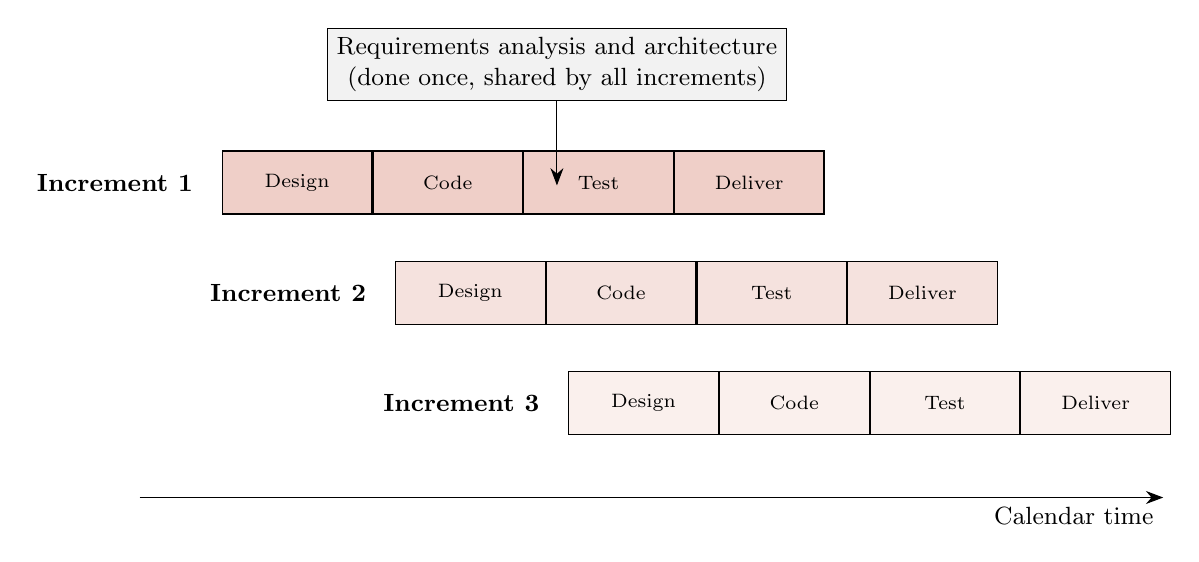
\begin{tikzpicture}[stage/.style={draw,minimum width=19mm,minimum height=8mm,font=\scriptsize,align=center}]
\foreach \y/\n/\c in {0/1/cgu!25,-1.4/2/cgu!15,-2.8/3/cgu!8}{
  \pgfmathsetmacro{\x}{(\n-1)*2.2}
  \node[font=\small\bfseries,anchor=east] at (\x-0.2,\y) {Increment \n};
  \node[stage,fill=\c] (a\n) at (\x+1,\y) {Design};
  \node[stage,fill=\c,right=0pt of a\n] (b\n) {Code};
  \node[stage,fill=\c,right=0pt of b\n] (c\n) {Test};
  \node[stage,fill=\c,right=0pt of c\n] (d\n) {Deliver};
}
\node[draw,fill=gray!10,minimum width=40mm,minimum height=8mm,font=\small,align=center] (req) at (4.3,1.5) {Requirements analysis and architecture\\ (done once, shared by all increments)};
\draw[arr] (req.south) -- ++(0,-1.07);
\draw[arr] (-1,-4) -- (12,-4) node[below left,font=\small] {Calendar time};
\end{tikzpicture}
\caption{Incremental development of SHMC}\label{fig:incremental}
\end{figure}

\begin{table}[H]
\centering\small
\caption{Increment plan}\label{tab:increments}
\begin{tabularx}{\textwidth}{clL}
\toprule
\textbf{No.} & \textbf{Target date} & \textbf{Modules delivered}\\
\midrule
1 & Week 15 & Authentication and RBAC, student profiles, hall and room inventory, room application, smart allotment engine, notices\\
2 & Week 23 & Fee structure, online payment and receipts, fines, mess menu and attendance, roommate compatibility\\
3 & Week 33 & Complaints with SLA escalation, leave and QR gate pass, visitor log, analytics dashboard, occupancy forecast\\
\bottomrule
\end{tabularx}
\end{table}

\section{Why Incremental Works Here}
\begin{itemize}
  \item \textbf{The calendar dictates priorities.} Allotment must work at semester start. Increment~1 is built around it, so the most time-critical feature ships first.
  \item \textbf{Requirements will move.} Mess rules, fines and leave policies vary between halls. Once wardens use Increment~1, they will tell us what they actually want from the later modules, and the model has room for that feedback.
  \item \textbf{Faults stay contained.} Each increment is tested on its own. A defect in the mess module cannot delay allotment.
  \item \textbf{Risk is moderate.} The technology is well known and the team is small. The heavy risk analysis of the spiral model would cost more than it saves.
  \item \textbf{Motivation.} A team that sees real users on its software after three months tends to stay motivated through the remaining two increments.
\end{itemize}

%================ CHAPTER 5 =================
\chapter{Software Requirements Specification}
This chapter follows the structure of IEEE Std 830-1998, adapted to the length of a case study.

\section{Introduction}
\subsection{Purpose}
This SRS describes the functional and non-functional requirements of the Students Hall Management Center, version 1.0. It is written for the development team, the project guide, and the hall administration who will accept the system.

\subsection{Definitions and Acronyms}
\begin{table}[H]
\centering\small
\caption{Definitions and acronyms}\label{tab:defs}
\begin{tabularx}{\textwidth}{lL}
\toprule
\textbf{Term} & \textbf{Meaning}\\
\midrule
Hall & A residential building for students, divided into blocks and floors\\
Allotment & Assignment of a specific bed in a room to a student for a session\\
Out-pass & Permission for a student to leave the campus for a period\\
SLA & Service Level Agreement: the maximum time allowed to resolve a complaint\\
RBAC & Role-Based Access Control\\
JWT & JSON Web Token, used for stateless authentication\\
HMAC & Hash-based Message Authentication Code, used to sign QR gate passes\\
PWA & Progressive Web App: a website that can be installed like a mobile app\\
\bottomrule
\end{tabularx}
\end{table}

\section{Overall Description}
\subsection{Product Perspective}
SHMC is a new, self-contained system. It exchanges data with three external systems: the Razorpay payment gateway, an SMTP/SMS provider for notifications, and (read-only) a CSV export of enrolled students from the academic section, used to verify that an applicant is a current student.

\subsection{User Classes}
\begin{table}[H]
\centering\small
\caption{User classes and characteristics}\label{tab:users}
\begin{tabularx}{\textwidth}{lcL}
\toprule
\textbf{User class} & \textbf{Approx. count} & \textbf{Characteristics}\\
\midrule
Student & 5,000+ & Frequent, mostly mobile use; low tolerance for complex forms\\
Warden / Hall admin & 1 per hall & Daily use; approves allotments, leaves; needs dashboards\\
Chief warden & 1 & Receives escalations; views university-wide reports\\
Accountant & 2--3 & Sets fees, verifies payments, tracks dues\\
Mess manager & 1 per mess & Updates menu, attendance and extra charges\\
Security guard & 2--4 per gate & Shift-based use on a phone; scans QR passes, logs visitors\\
\bottomrule
\end{tabularx}
\end{table}

\subsection{Operating Environment}
The server runs on Ubuntu 24.04 LTS with Node.js 20 and MySQL 8. Clients need a current version of Chrome, Firefox, Safari or Edge on desktop or mobile. The guard's scanning screen needs a phone with a camera.

\subsection{Design and Implementation Constraints}
\begin{itemize}
  \item Allotment must honour hall gender rules and room capacity at all times.
  \item Card data must never be stored; payment is delegated to the gateway.
  \item The system must remain usable on a 3G connection for the student and guard screens.
  \item All times are stored in UTC and displayed in IST.
\end{itemize}

\subsection{Assumptions and Dependencies}
\begin{itemize}
  \item The academic section supplies an up-to-date list of enrolled students each semester.
  \item Each hall has at least one warden with a smartphone or computer.
  \item Razorpay and the SMS provider are available with their published uptime.
\end{itemize}

\section{Functional Requirements}
Requirements are grouped by module. Priority follows MoSCoW: \textbf{M} = must have, \textbf{S} = should have, \textbf{C} = could have.

\subsection{Authentication and User Management}
\begin{table}[H]
\centering\small
\caption{Functional requirements: authentication}\label{tab:fr-auth}
\begin{tabularx}{\textwidth}{lLc}
\toprule
\textbf{ID} & \textbf{Requirement} & \textbf{Priority}\\
\midrule
FR1.1 & Users log in with roll number or staff ID and password & M\\
FR1.2 & Passwords are reset through a one-time code sent to the registered email & M\\
FR1.3 & After 5 failed logins the account is locked for 15 minutes & M\\
FR1.4 & Each user has exactly one role; screens and APIs are restricted by role & M\\
FR1.5 & Admin can create, deactivate and reassign staff accounts & M\\
FR1.6 & Students can update phone, address and guardian contact; roll number and name are read-only & S\\
\bottomrule
\end{tabularx}
\end{table}

\subsection{Room Allotment}
\begin{table}[H]
\centering\small
\caption{Functional requirements: room allotment}\label{tab:fr-room}
\begin{tabularx}{\textwidth}{lLc}
\toprule
\textbf{ID} & \textbf{Requirement} & \textbf{Priority}\\
\midrule
FR2.1 & Student submits one application per session with up to three ranked preferences (hall, room type) & M\\
FR2.2 & Student fills a lifestyle questionnaire used for roommate matching & S\\
FR2.3 & System computes a priority score for each application (Section~\ref{sec:allot}) & M\\
FR2.4 & Warden runs the allotment engine for a hall; the engine proposes a room for each application & M\\
FR2.5 & Warden reviews, overrides if necessary (with a mandatory reason), and publishes the allotment & M\\
FR2.6 & Unallotted applicants go to a waitlist ordered by score and are allotted automatically when a bed frees up & M\\
FR2.7 & Student can request a room transfer; warden approves or rejects & S\\
FR2.8 & Student vacates at session end; the bed becomes available after warden checks the room & M\\
FR2.9 & Warden sees live vacancy per hall, block, floor and room type & M\\
\bottomrule
\end{tabularx}
\end{table}

\subsection{Fees and Payments}
\begin{table}[H]
\centering\small
\caption{Functional requirements: fees}\label{tab:fr-fee}
\begin{tabularx}{\textwidth}{lLc}
\toprule
\textbf{ID} & \textbf{Requirement} & \textbf{Priority}\\
\midrule
FR3.1 & Accountant defines fee heads (hostel, mess, security deposit) per hall and room type & M\\
FR3.2 & On allotment, the system raises an invoice for the student & M\\
FR3.3 & Student pays online; payment status is confirmed through the gateway's signed webhook, not the browser redirect & M\\
FR3.4 & A PDF receipt with a unique number is generated and emailed & M\\
FR3.5 & Reminders are sent 7 days and 1 day before the due date; a late fine is added automatically after it & S\\
FR3.6 & Accountant can record an offline (bank challan) payment with a reference number & M\\
FR3.7 & Accountant can issue a refund against a payment, with approval by the chief warden & C\\
\bottomrule
\end{tabularx}
\end{table}

\subsection{Mess Management}
\begin{table}[H]
\centering\small
\caption{Functional requirements: mess}\label{tab:fr-mess}
\begin{tabularx}{\textwidth}{lLc}
\toprule
\textbf{ID} & \textbf{Requirement} & \textbf{Priority}\\
\midrule
FR4.1 & Mess manager publishes a weekly menu & M\\
FR4.2 & Students can opt out of meals at least 24 hours in advance for a rebate & S\\
FR4.3 & Mess manager records extra items, which are added to the student's monthly mess bill & M\\
FR4.4 & Students rate each meal from 1 to 5; weekly averages appear on the warden's dashboard & C\\
\bottomrule
\end{tabularx}
\end{table}

\subsection{Complaints}
\begin{table}[H]
\centering\small
\caption{Functional requirements: complaints}\label{tab:fr-comp}
\begin{tabularx}{\textwidth}{lLc}
\toprule
\textbf{ID} & \textbf{Requirement} & \textbf{Priority}\\
\midrule
FR5.1 & Student raises a complaint with category, description and an optional photo & M\\
FR5.2 & Each category has an SLA; the deadline is computed when the complaint is raised & M\\
FR5.3 & Warden assigns the complaint to a staff member & M\\
FR5.4 & Status follows the state machine in Figure~\ref{fig:state} & M\\
FR5.5 & If the SLA is breached, the complaint is escalated to the chief warden automatically & S\\
FR5.6 & Student confirms resolution or reopens within 48 hours; otherwise it closes automatically & S\\
\bottomrule
\end{tabularx}
\end{table}

\subsection{Leave, Gate Pass and Visitors}
\begin{table}[H]
\centering\small
\caption{Functional requirements: leave and gate}\label{tab:fr-gate}
\begin{tabularx}{\textwidth}{lLc}
\toprule
\textbf{ID} & \textbf{Requirement} & \textbf{Priority}\\
\midrule
FR6.1 & Student applies for leave with dates, destination and reason & M\\
FR6.2 & Guardian receives an SMS; warden approves or rejects & M\\
FR6.3 & On approval, the student receives a signed QR gate pass valid only for the leave period & M\\
FR6.4 & Guard scans the QR at exit and entry; the system records actual out and in times & M\\
FR6.5 & Late return (after pass expiry) is flagged to the warden & S\\
FR6.6 & Guard records visitor name, phone, ID type, student visited, in-time and out-time & M\\
FR6.7 & Visitors are not allowed in residential blocks after 8 pm; the system blocks such entries & S\\
\bottomrule
\end{tabularx}
\end{table}

\subsection{Notices, Reports and Analytics}
\begin{table}[H]
\centering\small
\caption{Functional requirements: reports}\label{tab:fr-rep}
\begin{tabularx}{\textwidth}{lLc}
\toprule
\textbf{ID} & \textbf{Requirement} & \textbf{Priority}\\
\midrule
FR7.1 & Warden posts notices to a hall, a block, or all residents & M\\
FR7.2 & Dashboard shows occupancy, pending dues, open complaints and students currently out & M\\
FR7.3 & Reports export to PDF and Excel & S\\
FR7.4 & System forecasts next session's room demand per hall (Section~\ref{sec:forecast}) & C\\
\bottomrule
\end{tabularx}
\end{table}

\section{Non-Functional Requirements}
\begin{table}[H]
\centering\small
\caption{Non-functional requirements}\label{tab:nfr}
\begin{tabularx}{\textwidth}{llL}
\toprule
\textbf{ID} & \textbf{Attribute} & \textbf{Requirement and measure}\\
\midrule
NFR1 & Performance & 95\% of API calls respond within 500 ms at 500 concurrent users; allotment of 1,000 applications completes in under 10 s\\
NFR2 & Availability & 99.5\% monthly uptime; 99.9\% during the two-week allotment window\\
NFR3 & Security & bcrypt (cost 12) password hashing; TLS 1.2+; JWT expiry 15 min with refresh tokens; OWASP Top 10 mitigations\\
NFR4 & Privacy & Contact details visible only to the student, their warden and the admin\\
NFR5 & Reliability & Nightly full backup and hourly binary-log backup; recovery point objective 1 hour\\
NFR6 & Usability & A first-time student completes a room application in under 5 minutes without help\\
NFR7 & Scalability & A new hall is added through configuration only, without code changes\\
NFR8 & Maintainability & Unit test coverage of at least 80\% on service-layer code; ESLint clean builds\\
NFR9 & Portability & Runs in Docker containers on any Linux host\\
NFR10 & Auditability & Every change to an allotment, payment or complaint status is logged with user and timestamp\\
\bottomrule
\end{tabularx}
\end{table}

\section{External Interface Requirements}
\paragraph{User interfaces.} A responsive React single-page application. Students and guards primarily use phones, so their screens are designed mobile-first. Staff dashboards are designed for a laptop screen.

\paragraph{Hardware interfaces.} The guard screen uses the phone camera through the browser's \texttt{getUserMedia} API to scan QR codes. No other hardware is required.

\paragraph{Software interfaces.} Razorpay Orders and Webhooks API; SMTP for email; an SMS gateway's HTTP API; MySQL 8 via the \texttt{mysql2} driver; Redis 7.

\paragraph{Communication interfaces.} HTTPS with JSON bodies for all client--server traffic. The gateway calls our webhook endpoint over HTTPS with an HMAC signature header.
%================ CHAPTER 6 =================
\chapter{Analysis Modelling}
This chapter models \emph{what} the system does, independent of how it will be built. We use UML use case, activity and state diagrams for behaviour, and structured-analysis DFDs for data movement.

Table~\ref{tab:diagidx} lists where each diagram required by the case study brief appears in this report.

\begin{table}[H]
\centering\small
\caption{Index of required diagrams}\label{tab:diagidx}
\begin{tabularx}{\textwidth}{lL}
\toprule
\textbf{Required diagram} & \textbf{Where it appears}\\
\midrule
Use case diagram & Figure~\ref{fig:usecase} (with include/extend in Figure~\ref{fig:ucrel})\\
Data flow diagram (DFD) & Level 0: Figure~\ref{fig:dfd0}; Level 1: Figure~\ref{fig:dfd1}; Level 2: Figure~\ref{fig:dfd2}\\
State machine diagram & Figure~\ref{fig:state}\\
Sequence diagram & Figures~\ref{fig:seqallot}, \ref{fig:seqpay} and \ref{fig:seqqr}\\
Flowchart & Figure~\ref{fig:flowchart} (allotment algorithm); activity flow in Figure~\ref{fig:activity}\\
Graph & Control flow graph: Figure~\ref{fig:flowgraph}; demand forecast graph: Figure~\ref{fig:forecast}; live occupancy graph in the app: Figure~\ref{fig:ss-dash}\\
Others & Class (Fig.~\ref{fig:class}), ER (Fig.~\ref{fig:er}), architecture (Fig.~\ref{fig:arch}), deployment (Fig.~\ref{fig:deploy}), Gantt (Fig.~\ref{fig:gantt})\\
\bottomrule
\end{tabularx}
\end{table}

\section{Use Case Diagram}
Figure~\ref{fig:usecase} shows the seven actors and their main use cases. Every actor first passes through \emph{Login}, which is left out of the drawing for clarity. The payment gateway acts as a secondary actor on \emph{Pay fees online}.

\begin{figure}[!htbp]
\centering
\resizebox{\textwidth}{!}{%
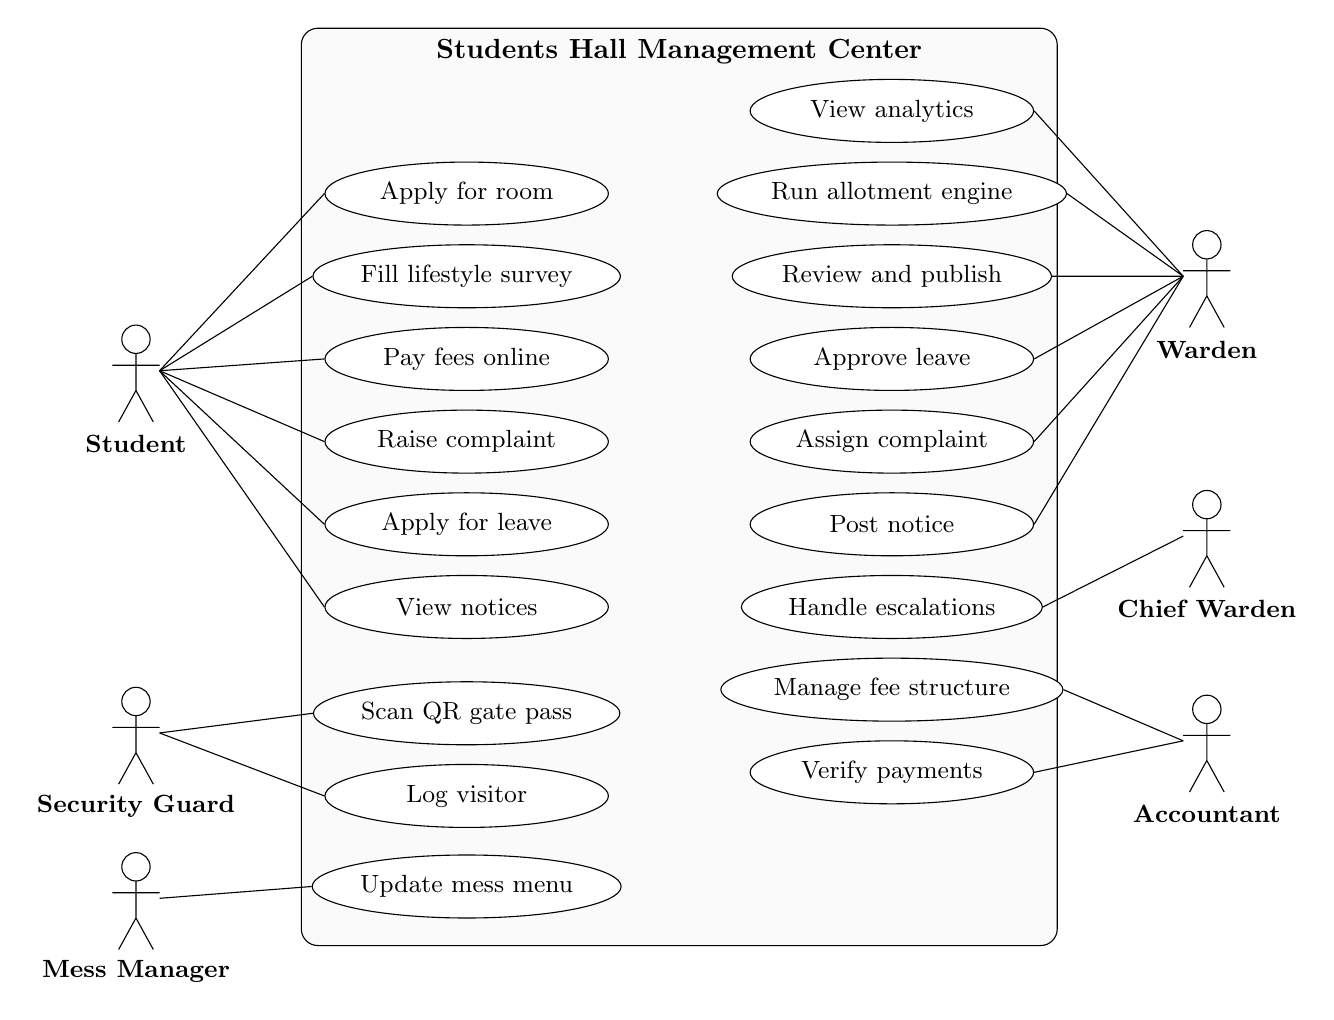
\begin{tikzpicture}
\draw[rounded corners=6pt,fill=gray!4] (2.9,2.1) rectangle (12.5,-9.55);
\node[font=\bfseries] at (7.7,1.8) {Students Hall Management Center};
% left column
\foreach \n/\y/\t in {L1/0/Apply for room,L2/-1.05/Fill lifestyle survey,L3/-2.1/Pay fees online,L4/-3.15/Raise complaint,L5/-4.2/Apply for leave,L6/-5.25/View notices,L7/-6.6/Scan QR gate pass,L8/-7.65/Log visitor,L9/-8.8/Update mess menu}
  \node[uc,fill=white] (\n) at (5,\y) {\t};
% right column
\foreach \n/\y/\t in {R0/1.05/View analytics,R1/0/Run allotment engine,R2/-1.05/Review and publish,R3/-2.1/Approve leave,R4/-3.15/Assign complaint,R5/-4.2/Post notice,R6/-5.25/Handle escalations,R7/-6.3/Manage fee structure,R8/-7.35/Verify payments}
  \node[uc,fill=white] (\n) at (10.4,\y) {\t};
\actor{st}{0.8,-2.4}{Student}
\actor{gd}{0.8,-7.0}{Security Guard}
\actor{ms}{0.8,-9.1}{Mess Manager}
\actor{wd}{14.4,-1.2}{Warden}
\actor{cw}{14.4,-4.5}{Chief Warden}
\actor{ac}{14.4,-7.1}{Accountant}
\foreach \u in {L1,L2,L3,L4,L5,L6} \draw ($(st)+(0.3,0)$) -- (\u.west);
\foreach \u in {L7,L8} \draw ($(gd)+(0.3,0)$) -- (\u.west);
\draw ($(ms)+(0.3,0)$) -- (L9.west);
\foreach \u in {R0,R1,R2,R3,R4,R5} \draw ($(wd)+(-0.3,0)$) -- (\u.east);
\foreach \u in {R6} \draw ($(cw)+(-0.3,0)$) -- (\u.east);
\foreach \u in {R7,R8} \draw ($(ac)+(-0.3,0)$) -- (\u.east);
\end{tikzpicture}}
\caption{Use case diagram of SHMC}\label{fig:usecase}
\end{figure}

Two use cases are refined further with \texttt{<<include>>} and \texttt{<<extend>>} relationships in Figure~\ref{fig:ucrel}. \emph{Pay fees online} always includes \emph{Generate receipt}; \emph{Resolve complaint} is extended by \emph{Escalate complaint} only when the SLA is breached.

\begin{figure}[!htbp]
\centering
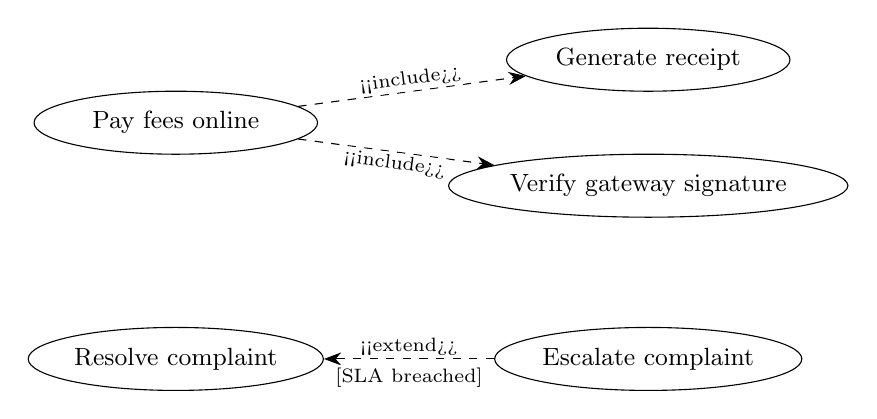
\begin{tikzpicture}
\node[uc] (pay) at (0,0) {Pay fees online};
\node[uc] (rec) at (6,0.8) {Generate receipt};
\node[uc] (ver) at (6,-0.8) {Verify gateway signature};
\draw[arr,dashed] (pay) -- node[lbl,above,sloped] {<<include>>} (rec);
\draw[arr,dashed] (pay) -- node[lbl,below,sloped] {<<include>>} (ver);
\node[uc] (res) at (0,-3) {Resolve complaint};
\node[uc] (esc) at (6,-3) {Escalate complaint};
\draw[arr,dashed] (esc) -- node[lbl,above] {<<extend>>} node[lbl,below,yshift=-2pt] {[SLA breached]} (res);
\end{tikzpicture}
\caption{Include and extend relationships}\label{fig:ucrel}
\end{figure}

\section{Use Case Specifications}
Four use cases carry most of the system's logic. Their full specifications follow.

\newcommand{\ucspec}[8]{%
\begin{table}[H]\centering\small\caption{#1}
\begin{tabularx}{\textwidth}{>{\bfseries}p{3.1cm}L}
\toprule
Actors & #2\\ Precondition & #3\\ Trigger & #4\\ Main flow & #5\\ Alternate flows & #6\\ Postcondition & #7\\ Related FRs & #8\\
\bottomrule
\end{tabularx}\end{table}}

\ucspec{UC-01: Apply for room}{Student (primary)}{Student is logged in, enrolled for the session and has no pending dues}
{Allotment window for the session is open}
{1. Student opens the application form. 2. System shows halls and room types permitted for the student's gender and year. 3. Student ranks up to three preferences. 4. Student completes the lifestyle questionnaire. 5. Student submits. 6. System validates, stores the application with status \emph{Submitted}, and shows an application ID.}
{3a. Student selects a room type not allowed for their year: system rejects the choice with a message. 5a. Student already has an application this session: system opens it for editing instead. 1a. Pending dues exist: system blocks the form and links to the payment page.}
{Application stored with status \emph{Submitted}; priority score computed}{FR2.1, FR2.2, FR2.3}

\ucspec{UC-02: Run allotment engine}{Warden (primary)}{Allotment window has closed; warden is logged in}
{Warden clicks \emph{Run allotment} for a hall}
{1. System locks the hall's vacancy data. 2. System sorts applications by priority score. 3. For each application, system tries preferences in order and picks the most compatible vacant bed (Algorithm~\ref{alg:allot}). 4. System shows proposed allotments and the waitlist. 5. Warden reviews and may override a proposal with a reason. 6. Warden publishes.}
{3a. No vacancy in any preference: application goes to the waitlist. 5a. Warden cancels: all proposals are discarded and the lock is released.}
{Allotments published, invoices raised, students notified by email}{FR2.4, FR2.5, FR2.6}

\ucspec{UC-03: Pay fees online}{Student (primary), Payment gateway (secondary)}{An unpaid invoice exists for the student}
{Student clicks \emph{Pay now}}
{1. System creates a gateway order for the invoice amount. 2. Gateway checkout opens. 3. Student pays. 4. Gateway calls the SHMC webhook with a signed payload. 5. System verifies the HMAC signature and amount. 6. System marks the invoice paid and generates a receipt (include: Generate receipt).}
{3a. Payment fails or is cancelled: invoice stays unpaid; student can retry. 4a. Webhook delayed: a reconciliation job polls the gateway every 10 minutes. 5a. Signature invalid: event is logged and ignored.}
{Invoice status \emph{Paid}; receipt emailed}{FR3.2, FR3.3, FR3.4}

\ucspec{UC-04: Raise complaint}{Student (primary), Warden, Staff}{Student is logged in and currently allotted a room}
{Student notices a problem in the room or hall}
{1. Student selects a category and writes a description. 2. Student optionally attaches a photo. 3. System stores the complaint with status \emph{Open} and computes the SLA deadline. 4. Warden is notified and assigns a staff member. 5. Staff resolves and marks \emph{Resolved}. 6. Student confirms; complaint closes.}
{5a. SLA deadline passes before resolution: complaint is escalated to the chief warden (extend: Escalate complaint). 6a. Student reopens within 48 hours: status returns to \emph{Assigned}.}
{Complaint closed with resolution time recorded}{FR5.1--FR5.6}

\section{Data Flow Diagrams}
\subsection{Level 0: Context Diagram}
At level 0 the whole system is one process. Figure~\ref{fig:dfd0} shows the six external entities and the data they exchange with it.

\begin{figure}[!htbp]
\centering
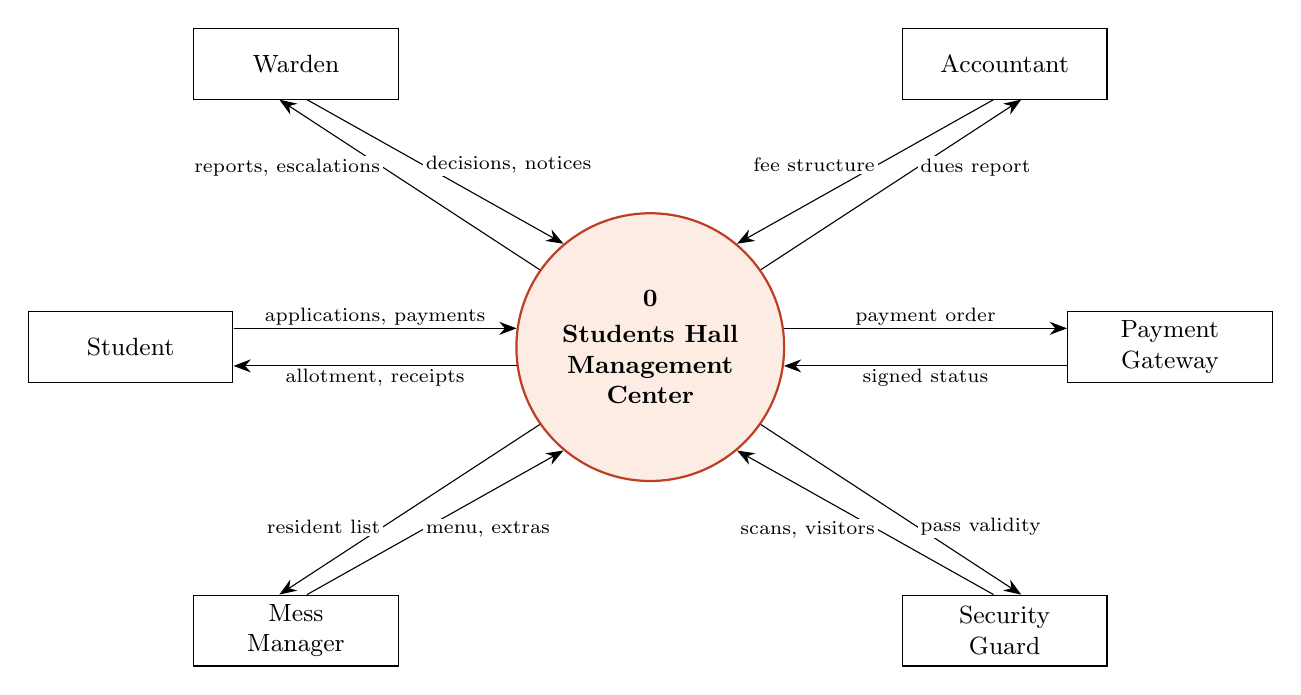
\begin{tikzpicture}[e/.style={ent,fill=white}]
\node[draw=cgu,fill=soft,thick,circle,minimum size=34mm,align=center,font=\small\bfseries] (p) at (0,0) {0\\[2pt]Students Hall\\Management\\Center};
\node[e] (s) at (-6.6,0) {Student};
\node[e] (g) at (6.6,0) {Payment\\Gateway};
\node[e] (w) at (-4.5,3.6) {Warden};
\node[e] (a) at (4.5,3.6) {Accountant};
\node[e] (m) at (-4.5,-3.6) {Mess\\Manager};
\node[e] (sg) at (4.5,-3.6) {Security\\Guard};
\draw[arr] (s.east |- p.172) -- node[lbl,above]{applications, payments} (p.172);
\draw[arr] (p.188) -- node[lbl,below]{allotment, receipts} (s.east |- p.188);
\draw[arr] (p.8) -- node[lbl,above]{payment order} (g.west |- p.8);
\draw[arr] (g.west |- p.352) -- node[lbl,below]{signed status} (p.352);
\draw[arr] ([xshift=4pt]w.south) -- node[lbl,right,pos=0.45]{decisions, notices} (p.130);
\draw[arr] (p.145) -- node[lbl,left,pos=0.6]{reports, escalations} ([xshift=-6pt]w.south);
\draw[arr] ([xshift=-4pt]a.south) -- node[lbl,left,pos=0.45]{fee structure} (p.50);
\draw[arr] (p.35) -- node[lbl,right,pos=0.6]{dues report} ([xshift=6pt]a.south);
\draw[arr] ([xshift=4pt]m.north) -- node[lbl,right,pos=0.45]{menu, extras} (p.230);
\draw[arr] (p.215) -- node[lbl,left,pos=0.6]{resident list} ([xshift=-6pt]m.north);
\draw[arr] ([xshift=-4pt]sg.north) -- node[lbl,left,pos=0.45]{scans, visitors} (p.310);
\draw[arr] (p.325) -- node[lbl,right,pos=0.6]{pass validity} ([xshift=6pt]sg.north);
\end{tikzpicture}
\caption{DFD Level 0 (context diagram)}\label{fig:dfd0}
\end{figure}

\subsection{Level 1}
Level 1 breaks the system into seven processes. Each owns one main data store; process 7.0 only reads from the others.

\begin{figure}[!htbp]
\centering
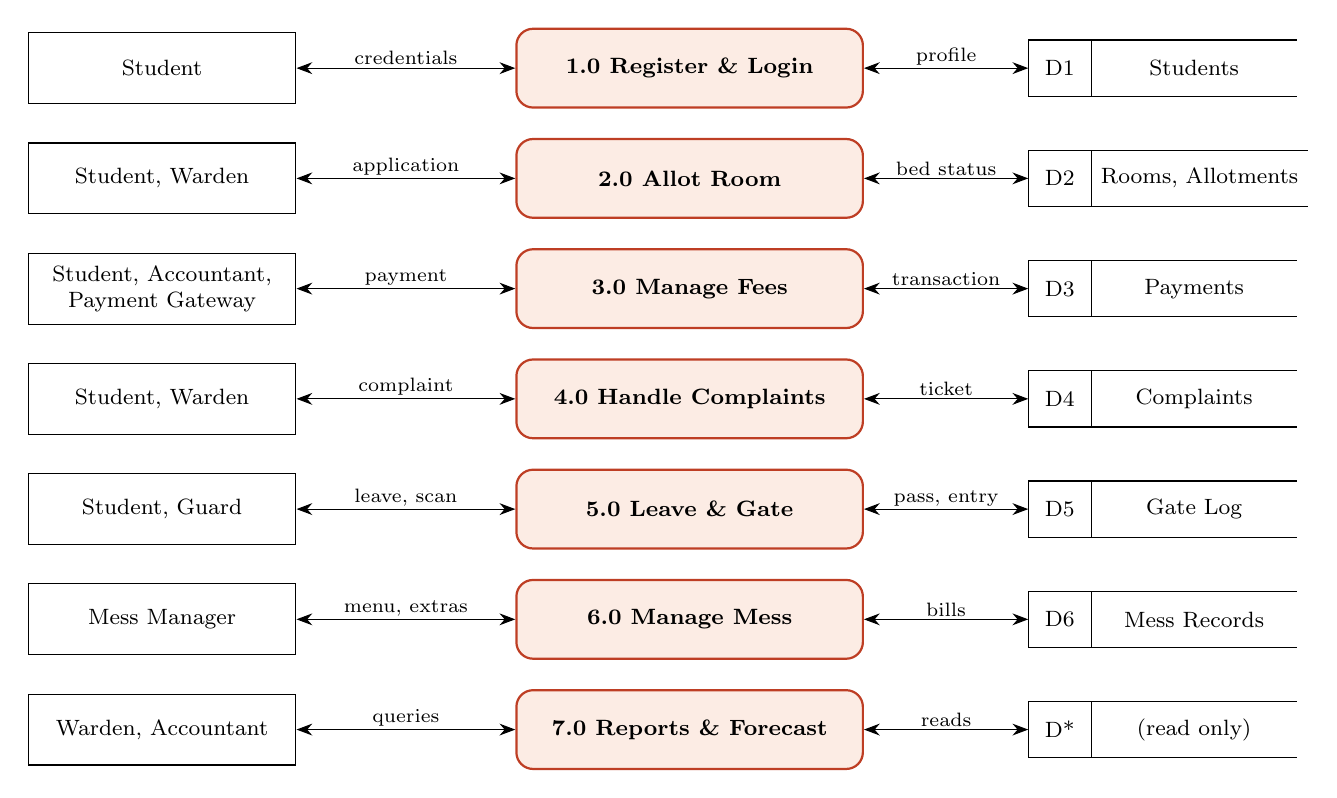
\begin{tikzpicture}[e/.style={ent,minimum width=34mm,font=\footnotesize,align=center},
  p/.style={proc,minimum width=44mm,font=\footnotesize\bfseries},
  lab/.style={font=\scriptsize,above,inner sep=1pt}]
\newcommand{\store}[3]{\node[minimum width=34mm,minimum height=7mm,font=\footnotesize,anchor=west] (#1) at (#2) {\hspace{8mm}#3};
  \draw ($(#1.north west)$) -- ($(#1.north east)$) ($(#1.south west)$) -- ($(#1.south east)$) ($(#1.north west)$) -- ($(#1.south west)$) ($(#1.north west)+(0.8,0)$) -- ($(#1.south west)+(0.8,0)$);}
\foreach \i/\y/\en/\pn/\sid/\sn/\fl/\fr in {
{1}/{0}/{Student}/{1.0 Register \& Login}/{D1}/{Students}/{credentials}/{profile},
{2}/{-1.4}/{Student, Warden}/{2.0 Allot Room}/{D2}/{Rooms, Allotments}/{application}/{bed status},
{3}/{-2.8}/{Student, Accountant,\\Payment Gateway}/{3.0 Manage Fees}/{D3}/{Payments}/{payment}/{transaction},
{4}/{-4.2}/{Student, Warden}/{4.0 Handle Complaints}/{D4}/{Complaints}/{complaint}/{ticket},
{5}/{-5.6}/{Student, Guard}/{5.0 Leave \& Gate}/{D5}/{Gate Log}/{leave, scan}/{pass, entry},
{6}/{-7.0}/{Mess Manager}/{6.0 Manage Mess}/{D6}/{Mess Records}/{menu, extras}/{bills},
{7}/{-8.4}/{Warden, Accountant}/{7.0 Reports \& Forecast}/{D*}/{(read only)}/{queries}/{reads}}{
  \node[e] (e\i) at (-1.3,\y) {\en};
  \node[p] (p\i) at (5.4,\y) {\pn};
  \store{s\i}{9.7,\y}{\sn}
  \node[font=\footnotesize] at ($(s\i.west)+(0.4,0)$) {\sid};
  \draw[{Stealth[length=2mm]}-{Stealth[length=2mm]}] (e\i.east) -- node[lab]{\fl} (p\i.west);
  \draw[{Stealth[length=2mm]}-{Stealth[length=2mm]}] (p\i.east) -- node[lab]{\fr} (s\i.west);
}
\end{tikzpicture}
\caption{DFD Level 1}\label{fig:dfd1}
\end{figure}

\subsection{Level 2: Process 2.0 (Allot Room)}
Room allotment is the most complex process, so it is decomposed once more in Figure~\ref{fig:dfd2}.

\begin{figure}[!htbp]
\centering
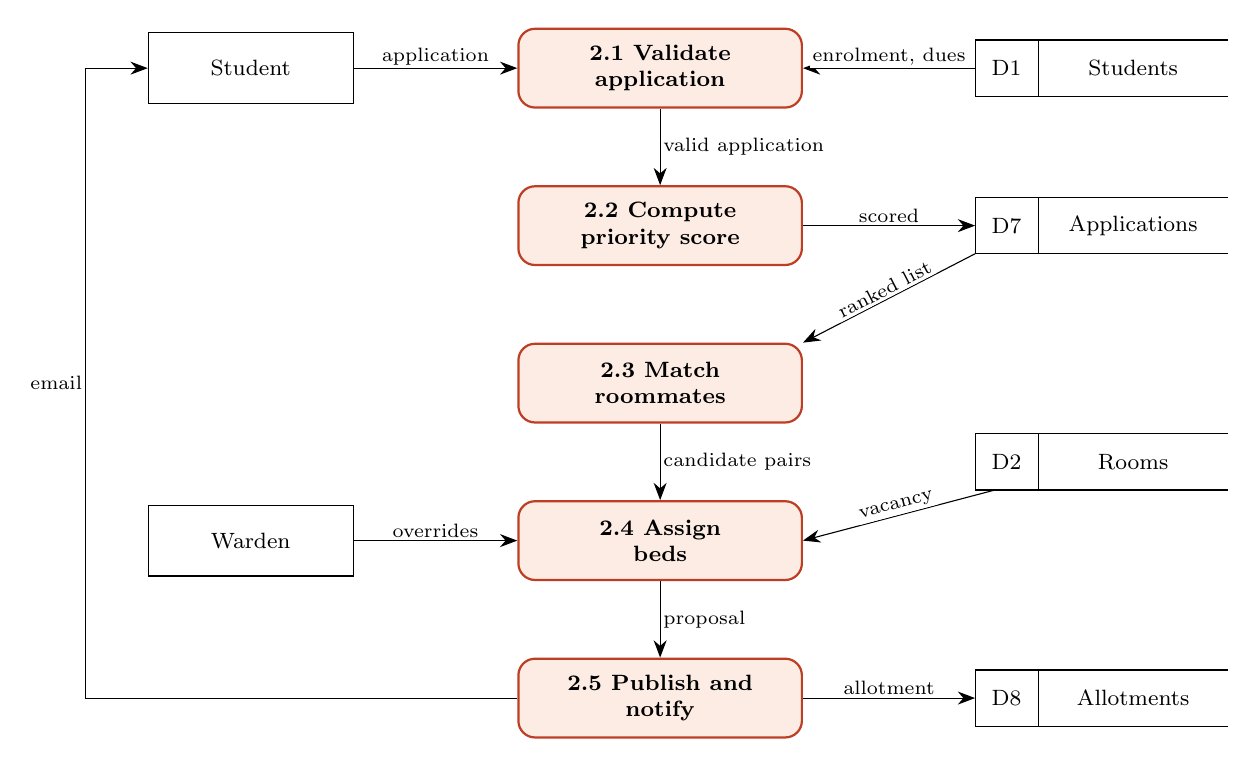
\begin{tikzpicture}[p/.style={proc,minimum width=36mm,font=\footnotesize\bfseries},
 lab/.style={font=\scriptsize,fill=white,inner sep=1pt}]
\newcommand{\store}[3]{\node[minimum width=32mm,minimum height=7mm,font=\footnotesize,anchor=west] (#1) at (#2) {\hspace{8mm}#3};
  \draw ($(#1.north west)$) -- ($(#1.north east)$) ($(#1.south west)$) -- ($(#1.south east)$) ($(#1.north west)$) -- ($(#1.south west)$) ($(#1.north west)+(0.8,0)$) -- ($(#1.south west)+(0.8,0)$);}
\node[ent,font=\footnotesize] (st) at (-5.2,0) {Student};
\node[p] (a) at (0,0) {2.1 Validate\\application};
\node[p] (b) at (0,-2) {2.2 Compute\\priority score};
\node[p] (c) at (0,-4) {2.3 Match\\roommates};
\node[p] (d) at (0,-6) {2.4 Assign\\beds};
\node[p] (e) at (0,-8) {2.5 Publish and\\notify};
\node[ent,font=\footnotesize] (wd) at (-5.2,-6) {Warden};
\store{d1}{4,0}{Students}\node[font=\footnotesize] at ($(d1.west)+(0.4,0)$) {D1};
\store{d7}{4,-2}{Applications}\node[font=\footnotesize] at ($(d7.west)+(0.4,0)$) {D7};
\store{d2}{4,-5}{Rooms}\node[font=\footnotesize] at ($(d2.west)+(0.4,0)$) {D2};
\store{d8}{4,-8}{Allotments}\node[font=\footnotesize] at ($(d8.west)+(0.4,0)$) {D8};
\draw[arr] (st) -- node[lab,above]{application} (a);
\draw[arr] (d1) -- node[lab,above]{enrolment, dues} (a);
\draw[arr] (a) -- node[lab,right]{valid application} (b);
\draw[arr] (b) -- node[lab,above]{scored} (d7);
\draw[arr] (d7.south west) -- node[lab,sloped,above]{ranked list} (c.north east);
\draw[arr] (c) -- node[lab,right]{candidate pairs} (d);
\draw[arr] (d2) -- node[lab,above,sloped]{vacancy} (d.east);
\draw[arr] (wd) -- node[lab,above]{overrides} (d);
\draw[arr] (d) -- node[lab,right]{proposal} (e);
\draw[arr] (e) -- node[lab,above]{allotment} (d8);
\draw[arr] (e.west) -- (-7.3,-8) |- node[lab,pos=0.25,left]{email} (st.west);
\end{tikzpicture}
\caption{DFD Level 2 for process 2.0}\label{fig:dfd2}
\end{figure}

\section{Activity Diagram: From Application to Allotment}
Figure~\ref{fig:activity} traces one student's application from submission to allotment, including the waitlist loop.

\begin{figure}[!htbp]
\centering
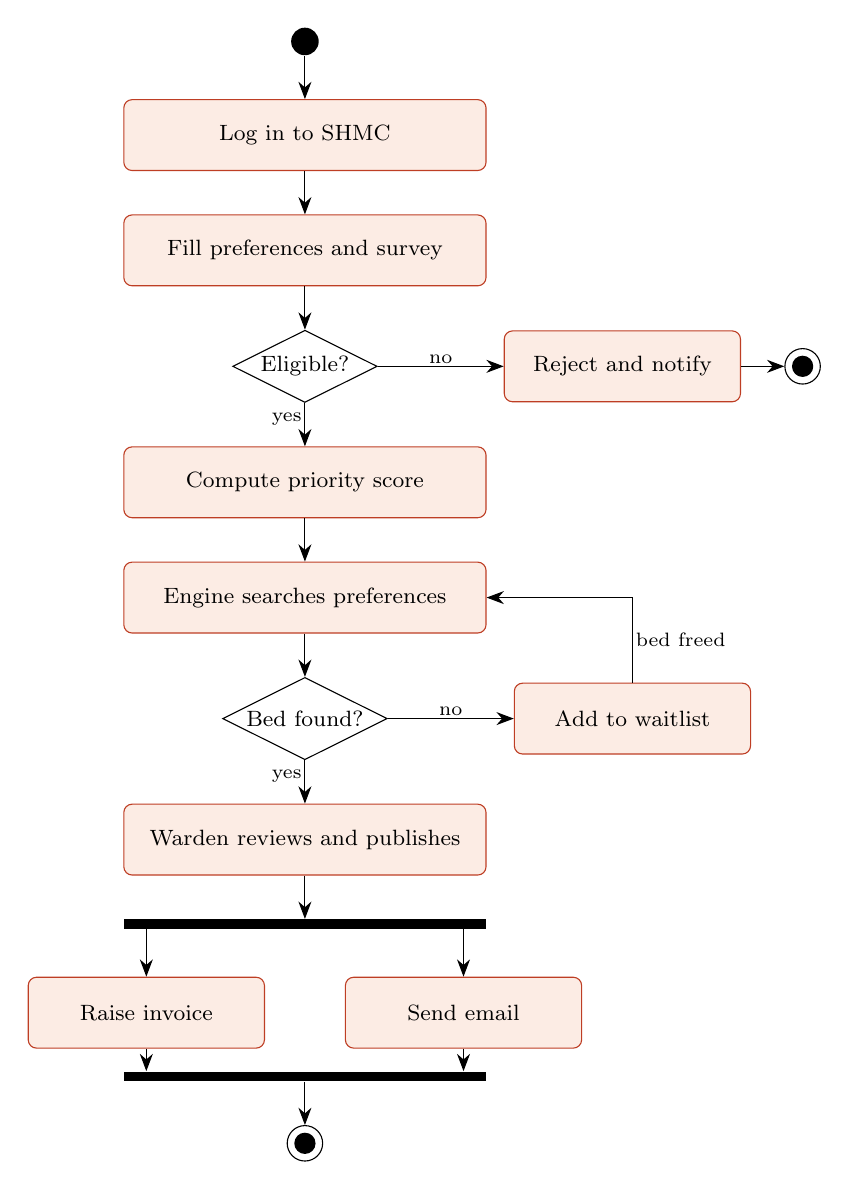
\begin{tikzpicture}[a/.style={box,fill=soft,draw=cgu,minimum width=46mm,font=\footnotesize},node distance=5.5mm]
\node[circle,fill=black,minimum size=3.5mm,inner sep=0] (s) {};
\node[a,below=of s] (n1) {Log in to SHMC};
\node[a,below=of n1] (n2) {Fill preferences and survey};
\node[dec,below=of n2,font=\footnotesize] (d1) {Eligible?};
\node[a,right=16mm of d1,minimum width=30mm] (rej) {Reject and notify};
\node[a,below=of d1] (n3) {Compute priority score};
\node[a,below=of n3] (n4) {Engine searches preferences};
\node[dec,below=of n4,font=\footnotesize] (d2) {Bed found?};
\node[a,right=16mm of d2,minimum width=30mm] (wl) {Add to waitlist};
\node[a,below=of d2] (n5) {Warden reviews and publishes};
\node[fill=black,minimum width=46mm,minimum height=1.2mm,inner sep=0,below=of n5] (fork) {};
\node[a,below left=6mm and -18mm of fork,minimum width=30mm] (inv) {Raise invoice};
\node[a,below right=6mm and -18mm of fork,minimum width=30mm] (mail) {Send email};
\node[fill=black,minimum width=46mm,minimum height=1.2mm,inner sep=0,below=18mm of fork] (join) {};
\node[circle,draw,minimum size=4.5mm,inner sep=0,below=of join] (e) {};
\node[circle,fill=black,minimum size=2.7mm,inner sep=0] at (e) {};
\node[circle,draw,minimum size=4.5mm,inner sep=0,right=of rej] (e2) {};
\node[circle,fill=black,minimum size=2.7mm,inner sep=0] at (e2) {};
\foreach \x/\y in {s/n1,n1/n2,n2/d1,d1/n3,n3/n4,n4/d2,d2/n5,n5/fork,join/e} \draw[arr] (\x) -- (\y);
\draw[arr] (d1) -- node[lbl,above]{no} (rej);
\draw[arr] (rej) -- (e2);
\draw[arr] (d2) -- node[lbl,above]{no} (wl);
\draw[arr] (wl.north) |- node[lbl,pos=0.25,right]{bed freed} (n4.east);
\node[lbl,left] at ($(d1.south)+(0,-0.2)$) {yes};
\node[lbl,left] at ($(d2.south)+(0,-0.2)$) {yes};
\draw[arr] (fork.south -| inv.north) -- (inv.north);
\draw[arr] (fork.south -| mail.north) -- (mail.north);
\draw[arr] (inv.south) -- (inv.south |- join.north);
\draw[arr] (mail.south) -- (mail.south |- join.north);
\end{tikzpicture}
\caption{Activity diagram: room application}\label{fig:activity}
\end{figure}

\section{State Machine Diagram: Complaint Lifecycle}
A complaint moves through seven states. The \emph{Escalated} state is entered automatically by a scheduled job when the SLA deadline passes.

\begin{figure}[!htbp]
\centering
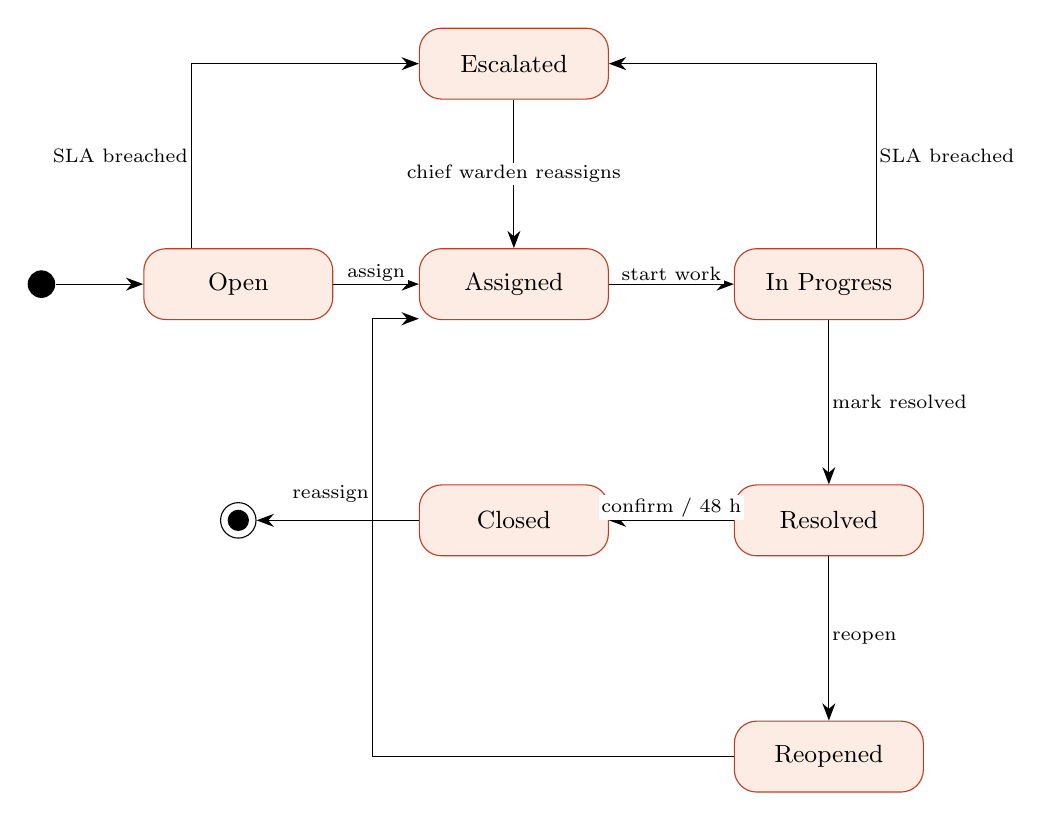
\begin{tikzpicture}[s/.style={draw,rounded corners=8pt,fill=soft,draw=cgu,minimum width=24mm,minimum height=9mm,font=\small},
 lab/.style={font=\scriptsize,fill=white,inner sep=1pt}]
\node[circle,fill=black,minimum size=3.5mm,inner sep=0] (i) at (-2,0) {};
\node[s] (o) at (0.5,0) {Open};
\node[s] (as) at (4,0) {Assigned};
\node[s] (ip) at (8,0) {In Progress};
\node[s] (r) at (8,-3) {Resolved};
\node[s] (c) at (4,-3) {Closed};
\node[s] (re) at (8,-6) {Reopened};
\node[s] (esc) at (4,2.8) {Escalated};
\node[circle,draw,minimum size=4.5mm,inner sep=0] (f) at (0.5,-3) {};
\node[circle,fill=black,minimum size=2.7mm,inner sep=0] at (f) {};
\draw[arr] (i) -- (o);
\draw[arr] (o) -- node[lab,above]{assign} (as);
\draw[arr] (as) -- node[lab,above]{start work} (ip);
\draw[arr] (ip) -- node[lab,right]{mark resolved} (r);
\draw[arr] (r) -- node[lab,above]{confirm / 48 h} (c);
\draw[arr] (r) -- node[lab,right]{reopen} (re);
\draw[arr] (re.west) -- (2.2,-6) |- node[lab,pos=0.3,left]{reassign} (as.200);
\draw[arr] (c) -- (f);
\draw[arr] ([xshift=6mm]ip.north) |- node[lab,pos=0.25,right]{SLA breached} (esc.east);
\draw[arr] ([xshift=-6mm]o.north) |- node[lab,pos=0.25,left]{SLA breached} (esc.west);
\draw[arr] (esc.south) -- node[lab]{chief warden reassigns} (as.north);
\end{tikzpicture}
\caption{State machine diagram of a complaint}\label{fig:state}
\end{figure}
%================ CHAPTER 7 =================
\chapter{System Design}
Analysis told us what SHMC must do. Design decides how: which parts the system is split into, where each part runs, and how data is stored.

\section{Architectural Design}
SHMC uses a \textbf{layered, service-oriented architecture} inside a single deployable application (a ``modular monolith''). Each business area is a separate service module with its own routes, logic and tables, but all modules run in one Node.js process. This keeps deployment simple for a small team while leaving a clean path to split a module out later if load demands it.

\begin{figure}[!htbp]
\centering
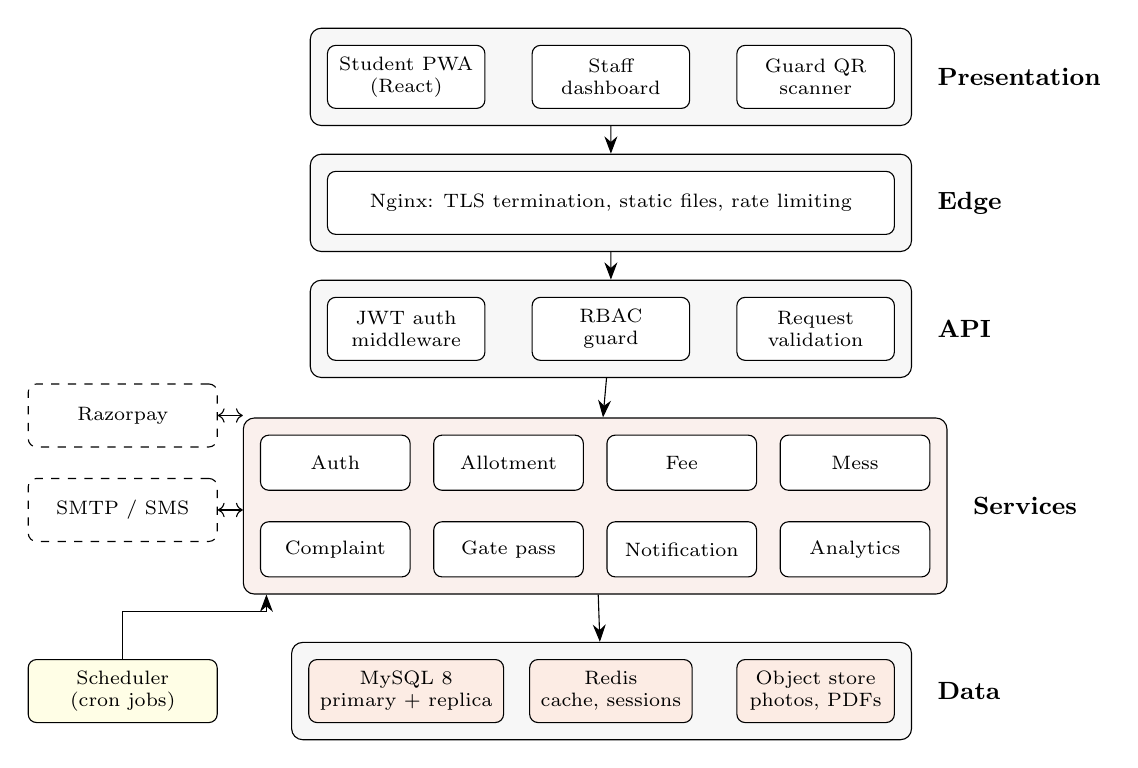
\begin{tikzpicture}[m/.style={box,fill=white,minimum width=20mm,font=\scriptsize,minimum height=8mm},
 layer/.style={draw,rounded corners=4pt,inner sep=6pt,fill=#1},
 ll/.style={font=\small\bfseries,anchor=west}]
% clients
\node[m] (c1) at (0,0) {Student PWA\\(React)};
\node[m] (c2) at (2.6,0) {Staff\\dashboard};
\node[m] (c3) at (5.2,0) {Guard QR\\scanner};
% gateway
\node[m,minimum width=72mm] (ng) at (2.6,-1.6) {Nginx: TLS termination, static files, rate limiting};
% api
\node[m] (a1) at (0,-3.2) {JWT auth\\middleware};
\node[m] (a2) at (2.6,-3.2) {RBAC\\guard};
\node[m] (a3) at (5.2,-3.2) {Request\\validation};
% services
\foreach \n/\x/\y/\t in {s1/-0.9/-4.9/Auth, s2/1.3/-4.9/Allotment, s3/3.5/-4.9/Fee, s4/5.7/-4.9/Mess, s5/-0.9/-6.0/Complaint, s6/1.3/-6.0/Gate pass, s7/3.5/-6.0/Notification, s8/5.7/-6.0/Analytics}
  \node[m,minimum width=19mm,minimum height=7mm] (\n) at (\x,\y) {\t};
% data
\node[m,fill=soft] (d1) at (0,-7.8) {MySQL 8\\primary + replica};
\node[m,fill=soft] (d2) at (2.6,-7.8) {Redis\\cache, sessions};
\node[m,fill=soft] (d3) at (5.2,-7.8) {Object store\\photos, PDFs};
\begin{scope}[on background layer]
\node[layer=gray!6,fit=(c1)(c3)] (L1) {};
\node[layer=gray!6,fit=(ng)] (L2) {};
\node[layer=gray!6,fit=(a1)(a3)] (L3) {};
\node[layer=cgu!8,fit=(s1)(s8)] (L4) {};
\node[layer=gray!6,fit=(d1)(d3)] (L5) {};
\end{scope}
\foreach \l/\t in {L1/Presentation,L2/Edge,L3/API,L4/Services,L5/Data} \node[ll] at ($(\l.east)+(0.2,0)$) {\t};
\draw[arr] (L1) -- (L2); \draw[arr] (L2) -- (L3); \draw[arr] (L3) -- (L4); \draw[arr] (L4) -- (L5);
% external + scheduler
\node[m,dashed,minimum width=24mm] (x1) at (-3.6,-4.3) {Razorpay};
\node[m,dashed,minimum width=24mm] (x2) at (-3.6,-5.5) {SMTP / SMS};
\node[m,minimum width=24mm,fill=yellow!10] (sch) at (-3.6,-7.8) {Scheduler\\(cron jobs)};
\draw[arr,<->] (x1) -- (L4.west |- x1);
\draw[arr,<->] (x2) -- (L4.west |- x2);
\draw[arr] (sch.north) -- ++(0,0.6) -| ($(L4.south west)+(0.3,0)$);
\end{tikzpicture}
\caption{Layered architecture of SHMC}\label{fig:arch}
\end{figure}

\paragraph{Presentation layer.} A React single-page application built as a PWA. Students and guards can install it on their phones. The guard view works offline for QR verification (Section~\ref{sec:qr}).

\paragraph{Edge layer.} Nginx terminates TLS, serves the compiled front end, and applies rate limits (for example, 10 login attempts per minute per IP).

\paragraph{API layer.} Express middleware verifies the JWT, checks the user's role against the route's permission, and validates the request body against a JSON schema before any service code runs.

\paragraph{Service layer.} Eight modules hold all business logic. Modules talk to each other through function calls and a small in-process event bus. For example, \emph{Allotment} emits \texttt{allotment.published}, which \emph{Fee} uses to raise an invoice and \emph{Notification} uses to send an email.

\paragraph{Data layer.} MySQL holds all transactional data. Redis caches vacancy counts and dashboards, and stores refresh tokens. Complaint photos and receipt PDFs go to object storage.

\paragraph{Scheduler.} Background jobs run on a timer: SLA checks every 15 minutes, fee reminders daily at 9 am, payment reconciliation every 10 minutes, and the demand forecast nightly.

\section{Design Principles Applied}
\begin{itemize}
  \item \textbf{High cohesion, low coupling.} Each service owns its tables. Other services read them only through the owning service's functions, never with direct SQL.
  \item \textbf{Separation of concerns.} Controllers handle HTTP only; services hold rules; repositories hold SQL.
  \item \textbf{Open--closed.} Allotment weights, SLA hours and fee heads are configuration rows, so policy changes need no code change (NFR7).
  \item \textbf{Fail safe.} Payment status is set only from the gateway's signed webhook, never from the browser, so a user cannot fake a successful payment.
\end{itemize}

\section{Deployment Design}
\begin{figure}[!htbp]
\centering
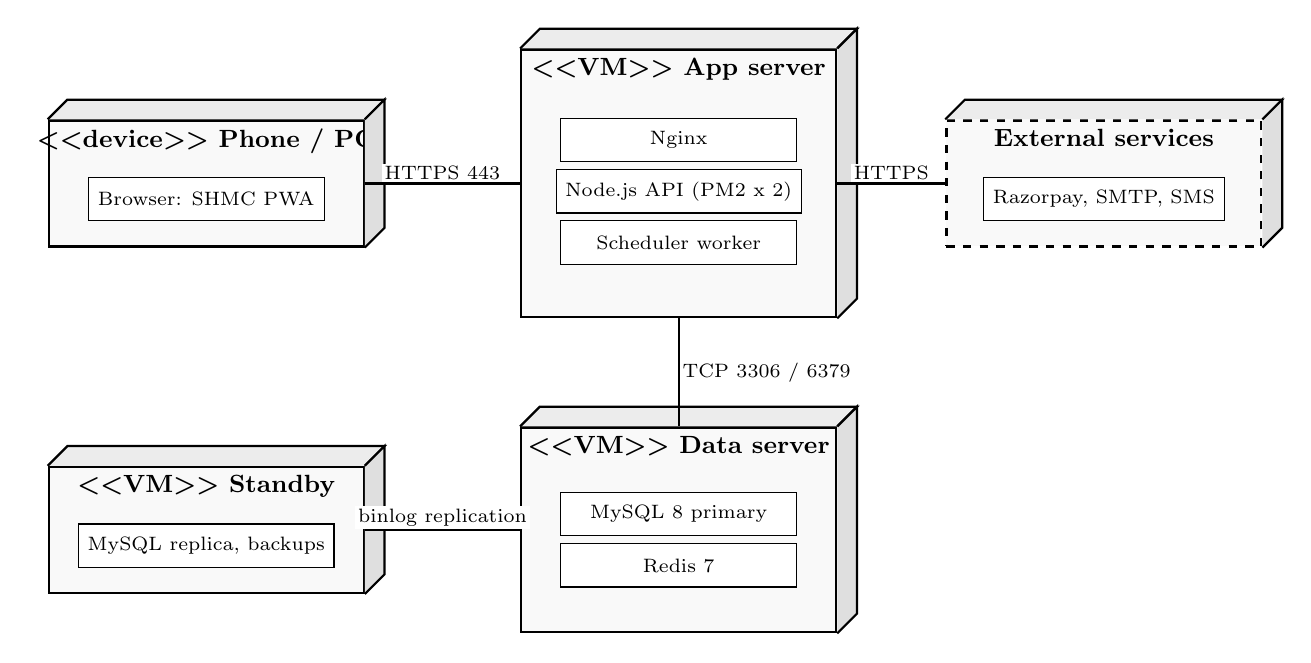
\begin{tikzpicture}[nd/.style={draw,thick,minimum width=40mm,minimum height=24mm,align=center,font=\small,fill=gray!5},
 art/.style={draw,fill=white,font=\scriptsize,minimum width=30mm,minimum height=5.5mm}]
\newcommand{\cube}[1]{\draw[thick,fill=gray!15] (#1.north west) -- ++(0.25,0.25) -- ($(#1.north east)+(0.25,0.25)$) -- (#1.north east); \draw[thick,fill=gray!25] (#1.north east) -- ++(0.25,0.25) -- ($(#1.south east)+(0.25,0.25)$) -- (#1.south east);}
\node[nd,minimum height=16mm] (cl) at (0,0) {};
\node[font=\small\bfseries,anchor=north] at (cl.north) {\textless\textless device\textgreater\textgreater\ Phone / PC};
\node[art] at ($(cl.center)+(0,-0.2)$) {Browser: SHMC PWA};
\node[nd,minimum height=34mm] (app) at (6,0) {};
\node[font=\small\bfseries,anchor=north] at (app.north) {\textless\textless VM\textgreater\textgreater\ App server};
\node[art] at ($(app.center)+(0,0.55)$) {Nginx};
\node[art] at ($(app.center)+(0,-0.1)$) {Node.js API (PM2 x 2)};
\node[art] at ($(app.center)+(0,-0.75)$) {Scheduler worker};
\node[nd,minimum height=26mm] (db) at (6,-4.4) {};
\node[font=\small\bfseries,anchor=north] at (db.north) {\textless\textless VM\textgreater\textgreater\ Data server};
\node[art] at ($(db.center)+(0,0.2)$) {MySQL 8 primary};
\node[art] at ($(db.center)+(0,-0.45)$) {Redis 7};
\node[nd,minimum height=16mm] (rep) at (0,-4.4) {};
\node[font=\small\bfseries,anchor=north] at (rep.north) {\textless\textless VM\textgreater\textgreater\ Standby};
\node[art] at ($(rep.center)+(0,-0.2)$) {MySQL replica, backups};
\node[nd,minimum height=16mm,dashed] (ext) at (11.4,0) {};
\node[font=\small\bfseries,anchor=north] at (ext.north) {External services};
\node[art] at ($(ext.center)+(0,-0.2)$) {Razorpay, SMTP, SMS};
\foreach \n in {cl,app,db,rep,ext} \cube{\n}
\draw[thick] (cl) -- node[lbl,above]{HTTPS 443} (app);
\draw[thick] (app) -- node[lbl,right]{TCP 3306 / 6379} (db);
\draw[thick] (db) -- node[lbl,above]{binlog replication} (rep);
\draw[thick] (app) -- node[lbl,above]{HTTPS} (ext);
\end{tikzpicture}
\caption{Deployment diagram}\label{fig:deploy}
\end{figure}

The app server and data server are separate VMs so that a spike in API traffic during allotment week cannot starve the database of memory. The standby VM receives binlog replication and holds nightly backups, which meets the one-hour recovery point objective in NFR5.

\section{Class Diagram}
Figure~\ref{fig:class} shows the main domain classes. The four user roles inherit from an abstract \texttt{User}. \texttt{AllotmentEngine} and \texttt{GatePassService} are service classes that hold the advanced logic described in Chapter~8.

\begin{figure}[!htbp]
\centering
\resizebox{\textwidth}{!}{%
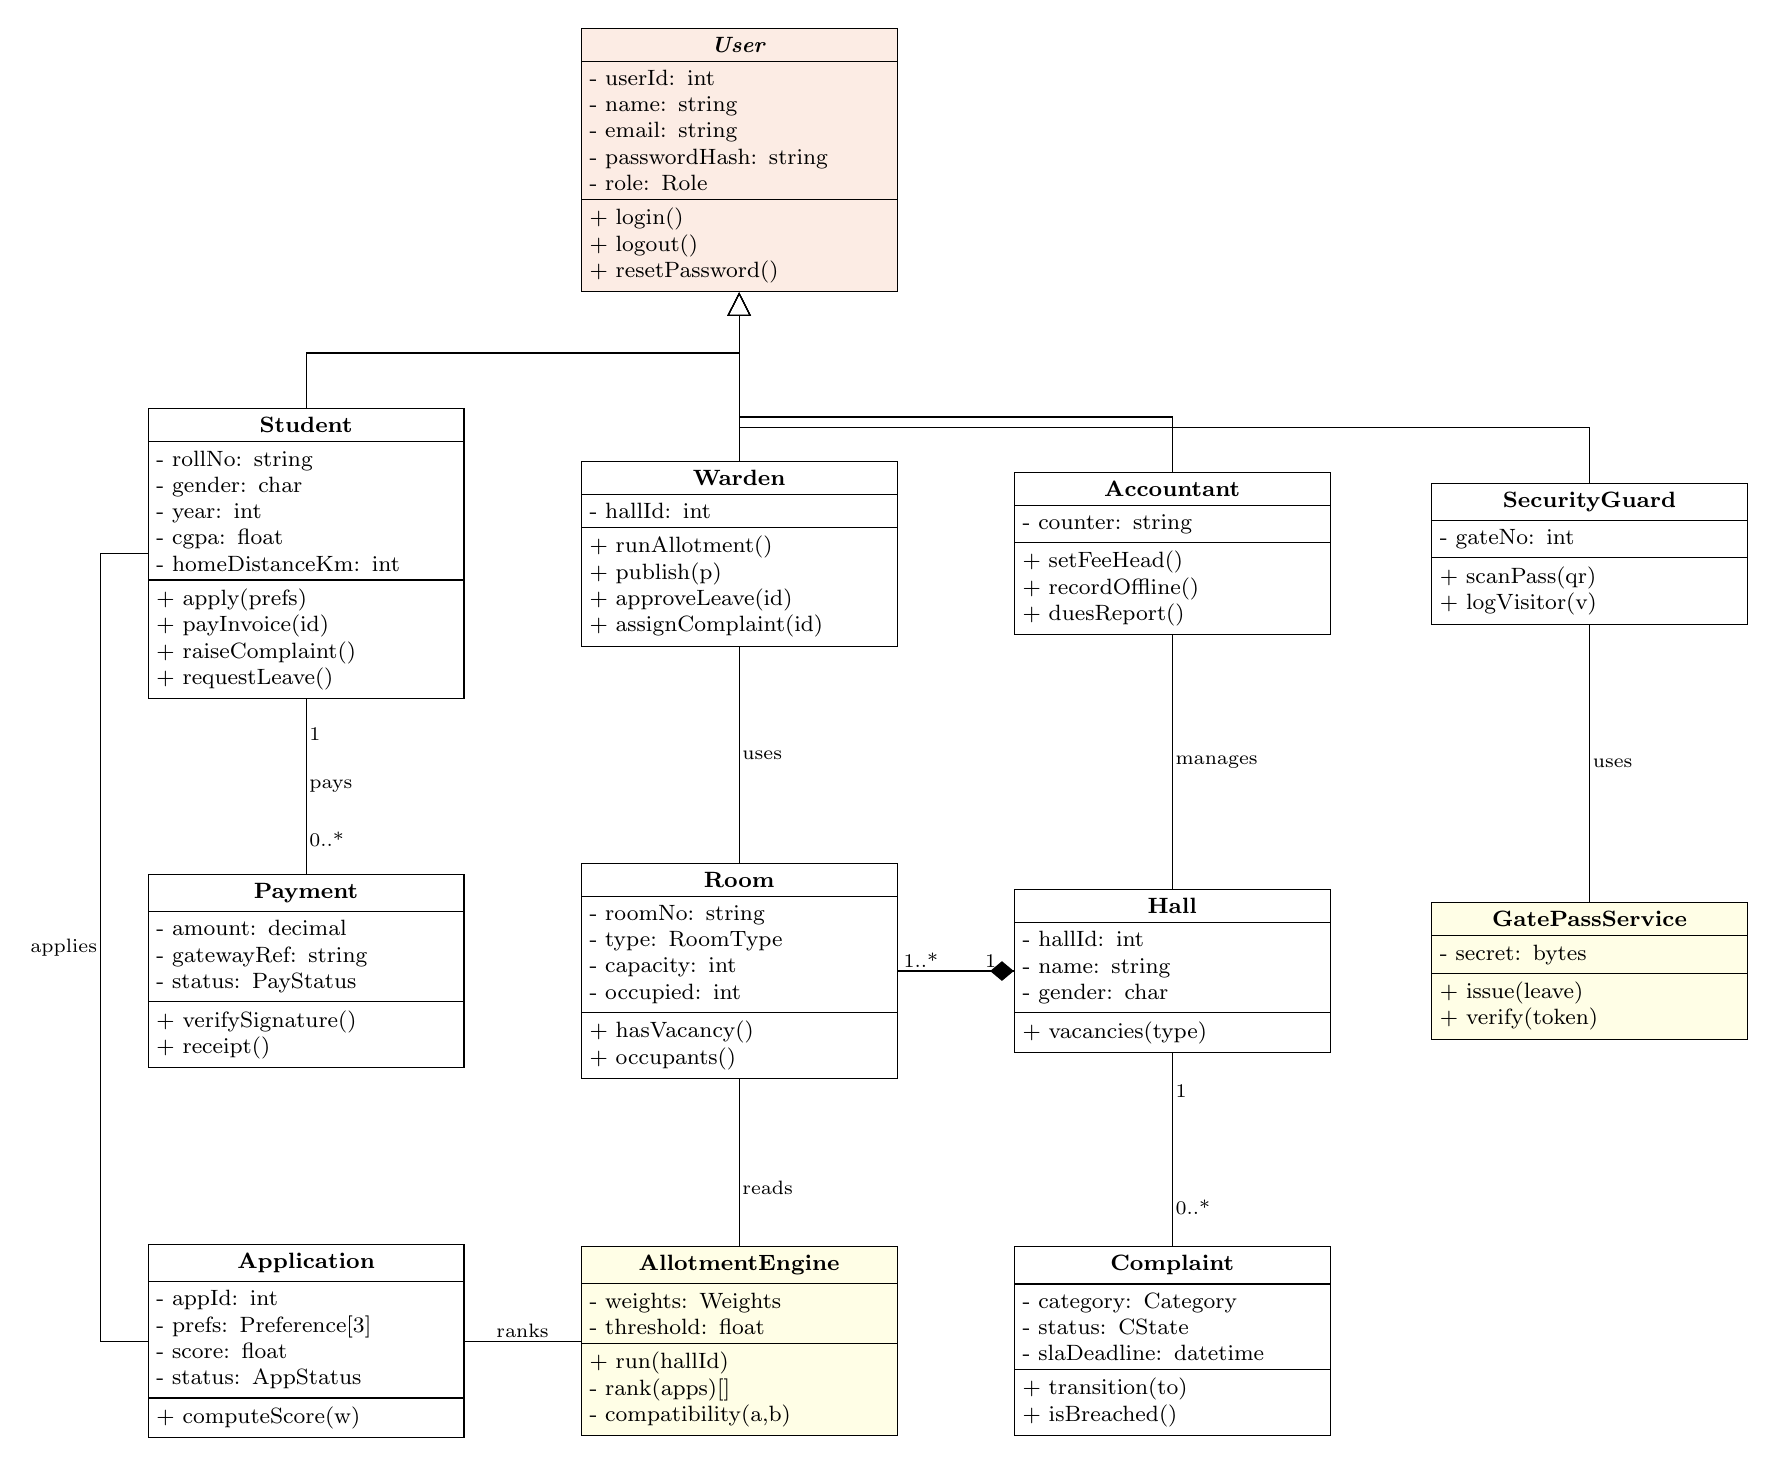
\begin{tikzpicture}[
 cls/.style={draw,rectangle split,rectangle split parts=3,font=\footnotesize,align=left,text width=38mm,fill=white,inner sep=3pt},
 inh/.style={-{Triangle[open,length=3mm,width=3mm]}},
 asc/.style={thin},
 lab/.style={font=\scriptsize,fill=white,inner sep=1pt}]
\node[cls,fill=soft] (user) at (5.5,0) {\hfil\textbf{\textit{User}}\hfil\nodepart{second}- userId: int\\- name: string\\- email: string\\- passwordHash: string\\- role: Role\nodepart{third}+ login()\\+ logout()\\+ resetPassword()};
\node[cls] (stu) at (0,-5) {\hfil\textbf{Student}\hfil\nodepart{second}- rollNo: string\\- gender: char\\- year: int\\- cgpa: float\\- homeDistanceKm: int\nodepart{third}+ apply(prefs)\\+ payInvoice(id)\\+ raiseComplaint()\\+ requestLeave()};
\node[cls] (war) at (5.5,-5) {\hfil\textbf{Warden}\hfil\nodepart{second}- hallId: int\nodepart{third}+ runAllotment()\\+ publish(p)\\+ approveLeave(id)\\+ assignComplaint(id)};
\node[cls] (acc) at (11,-5) {\hfil\textbf{Accountant}\hfil\nodepart{second}- counter: string\nodepart{third}+ setFeeHead()\\+ recordOffline()\\+ duesReport()};
\node[cls] (grd) at (16.3,-5) {\hfil\textbf{SecurityGuard}\hfil\nodepart{second}- gateNo: int\nodepart{third}+ scanPass(qr)\\+ logVisitor(v)};
\foreach \c in {stu,war,acc,grd} \draw[inh] (\c.north) -- ++(0,0.7) -| (user.south);
\node[cls] (app) at (0,-15) {\hfil\textbf{Application}\hfil\nodepart{second}- appId: int\\- prefs: Preference[3]\\- score: float\\- status: AppStatus\nodepart{third}+ computeScore(w)};
\node[cls] (room) at (5.5,-10.3) {\hfil\textbf{Room}\hfil\nodepart{second}- roomNo: string\\- type: RoomType\\- capacity: int\\- occupied: int\nodepart{third}+ hasVacancy()\\+ occupants()};
\node[cls] (hall) at (11,-10.3) {\hfil\textbf{Hall}\hfil\nodepart{second}- hallId: int\\- name: string\\- gender: char\nodepart{third}+ vacancies(type)};
\node[cls,fill=yellow!10] (eng) at (5.5,-15) {\hfil\textbf{AllotmentEngine}\hfil\nodepart{second}- weights: Weights\\- threshold: float\nodepart{third}+ run(hallId)\\- rank(apps)[]\\- compatibility(a,b)};
\node[cls] (cmp) at (11,-15) {\hfil\textbf{Complaint}\hfil\nodepart{second}- category: Category\\- status: CState\\- slaDeadline: datetime\nodepart{third}+ transition(to)\\+ isBreached()};
\node[cls,fill=yellow!10] (gps) at (16.3,-10.3) {\hfil\textbf{GatePassService}\hfil\nodepart{second}- secret: bytes\nodepart{third}+ issue(leave)\\+ verify(token)};
\node[cls] (pay) at (0,-10.3) {\hfil\textbf{Payment}\hfil\nodepart{second}- amount: decimal\\- gatewayRef: string\\- status: PayStatus\nodepart{third}+ verifySignature()\\+ receipt()};
\draw[asc] (stu.south) -- node[lab,pos=0.2,right]{1} node[lab,pos=0.8,right]{0..*} node[lab,pos=0.5,right]{pays} (pay.north);
\draw[asc] (hall.west) -- node[lab,pos=0.2,above]{1} node[lab,pos=0.8,above]{1..*} (room.east);
\draw[{Diamond[length=3mm,width=2.5mm]}-] (hall.west) -- (room.east);
\draw[asc] (war.south) -- node[lab,right]{uses} (room.north);
\draw[asc] (eng.north) -- node[lab,right,pos=0.35]{reads} (room.south);
\draw[asc] (eng.west) -- node[lab,above]{ranks} (eng.west -| app.east);
\draw[asc] (grd.south) -- node[lab,right]{uses} (gps.north);
\draw[asc] (hall.south) -- node[lab,pos=0.2,right]{1} node[lab,pos=0.8,right]{0..*} (cmp.north);
\draw[asc] (acc.south) -- node[lab,right]{manages} (hall.north);
\draw[asc] (stu.west) -- ++(-0.6,0) |- node[lab,pos=0.25,left]{applies} (app.west);
\end{tikzpicture}}
\caption{Class diagram}\label{fig:class}
\end{figure}

\section{Sequence Diagrams}
\subsection{Room Allotment}
Figure~\ref{fig:seqallot} shows the interaction when a student applies and, later, the warden runs the engine and publishes. The engine call is synchronous; the invoice and email are triggered through events after publication.

\begin{figure}[!htbp]
\centering
\resizebox{\textwidth}{!}{%
\begin{sequencediagram}
\newthread{s}{:Student}
\newinst[1.2]{ui}{:WebApp}
\newinst[1.2]{api}{:AllotmentService}
\newinst[1.2]{eng}{:AllotmentEngine}
\newinst[1.2]{db}{:Database}
\newinst[1.2]{w}{:Warden}
\begin{call}{s}{submit(prefs, survey)}{ui}{application ID}
  \begin{call}{ui}{POST /applications}{api}{201 Created}
    \begin{call}{api}{checkEligibility()}{db}{ok}\end{call}
    \begin{callself}{api}{computeScore()}{score}\end{callself}
    \begin{call}{api}{insert(application)}{db}{appId}\end{call}
  \end{call}
\end{call}
\begin{call}{w}{runAllotment(hall)}{api}{proposal}
  \begin{call}{api}{run(hallId)}{eng}{proposal}
    \begin{call}{eng}{rankedApps, vacancies}{db}{rows}\end{call}
    \begin{callself}{eng}{match and assign}{}\end{callself}
  \end{call}
\end{call}
\begin{call}{w}{publish(proposal)}{api}{done}
  \begin{call}{api}{commit allotments}{db}{ok}\end{call}
\end{call}
\mess{api}{event: allotment.published}{s}
\end{sequencediagram}}
\caption{Sequence diagram: room allotment}\label{fig:seqallot}
\end{figure}

\subsection{Online Fee Payment}
The key design decision in Figure~\ref{fig:seqpay} is that SHMC trusts only the gateway's server-to-server webhook. The browser redirect after checkout is used only to show a ``processing'' message.

\begin{figure}[!htbp]
\centering
\resizebox{\textwidth}{!}{%
\begin{sequencediagram}
\newthread{s}{:Student}
\newinst[1.4]{ui}{:WebApp}
\newinst[1.4]{fee}{:FeeService}
\newinst[1.4]{gw}{:Razorpay}
\newinst[1.4]{db}{:Database}
\begin{call}{s}{Pay now}{ui}{receipt shown}
  \begin{call}{ui}{POST /payments/order}{fee}{orderId}
    \begin{call}{fee}{create order(amount)}{gw}{orderId}\end{call}
    \begin{call}{fee}{save(PENDING)}{db}{ok}\end{call}
  \end{call}
  \begin{call}{ui}{open checkout}{gw}{redirect}\end{call}
\end{call}
\begin{call}{gw}{webhook(payload, signature)}{fee}{200 OK}
  \begin{callself}{fee}{verify HMAC}{valid}\end{callself}
  \begin{call}{fee}{update(PAID), receipt}{db}{ok}\end{call}
\end{call}
\end{sequencediagram}}
\caption{Sequence diagram: online fee payment}\label{fig:seqpay}
\end{figure}

\section{Database Design}
\subsection{ER Diagram}
The ER model in Figure~\ref{fig:er} has eleven entities. \textsf{STUDENT} is the hub: applications, allotments, payments, complaints, leave requests and visitors all reference it.

\begin{figure}[H]
\centering
\resizebox{\textwidth}{!}{%
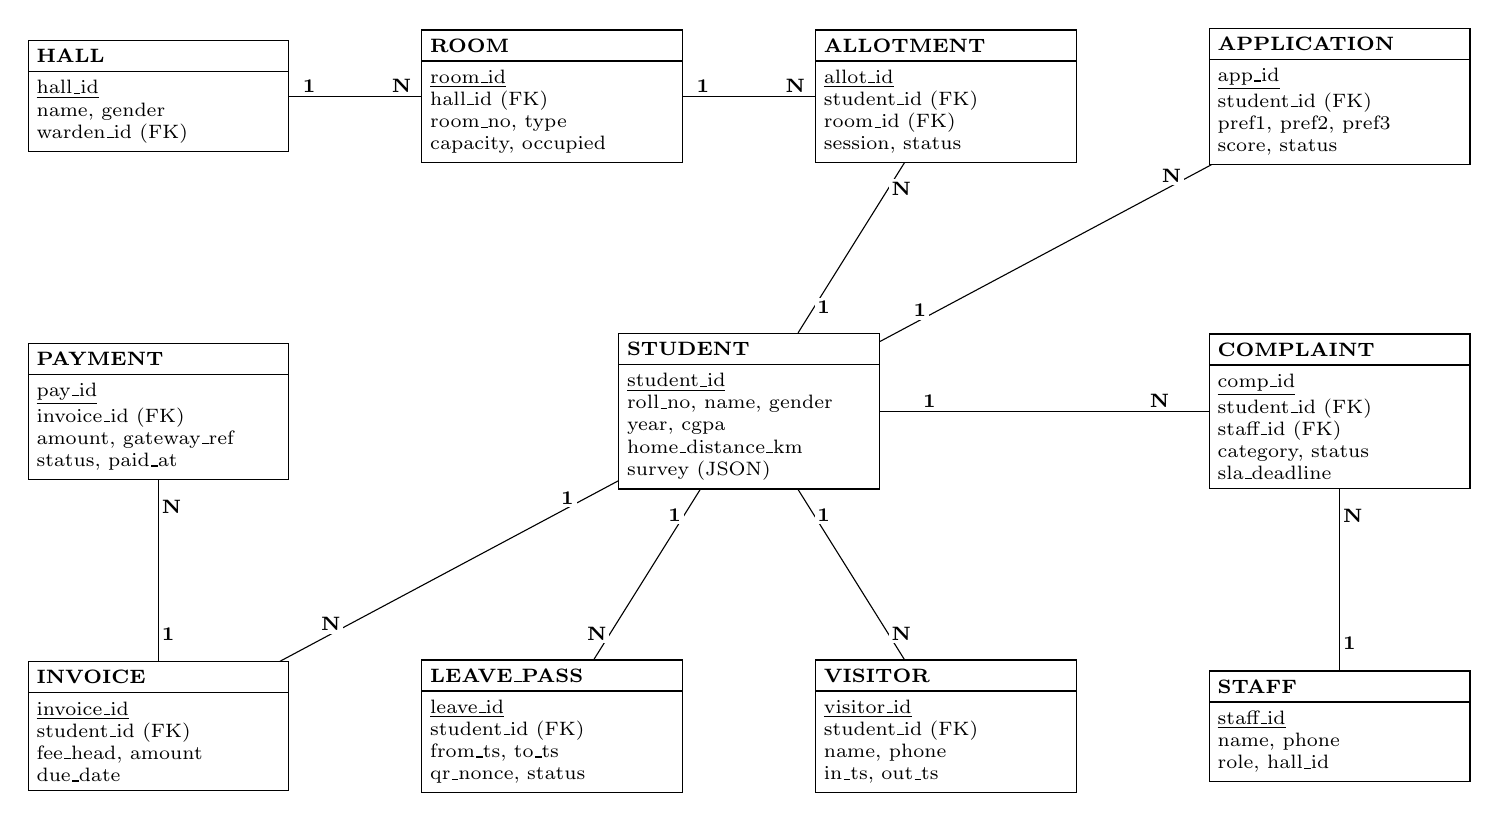
\begin{tikzpicture}[e/.style={draw,rectangle split,rectangle split parts=2,font=\scriptsize,text width=31mm,align=left,inner sep=3pt,fill=white},
 lab/.style={font=\scriptsize\bfseries,fill=white,inner sep=1pt}]
\newcommand{\ee}[4]{\node[e] (#1) at (#2) {\centering\textbf{#3}\nodepart{second}#4};}
\ee{hall}{0,0}{HALL}{\underline{hall\_id}\\name, gender\\warden\_id (FK)}
\ee{room}{5,0}{ROOM}{\underline{room\_id}\\hall\_id (FK)\\room\_no, type\\capacity, occupied}
\ee{allot}{10,0}{ALLOTMENT}{\underline{allot\_id}\\student\_id (FK)\\room\_id (FK)\\session, status}
\ee{app}{15,0}{APPLICATION}{\underline{app\_id}\\student\_id (FK)\\pref1, pref2, pref3\\score, status}
\ee{pay}{0,-4}{PAYMENT}{\underline{pay\_id}\\invoice\_id (FK)\\amount, gateway\_ref\\status, paid\_at}
\ee{inv}{0,-8}{INVOICE}{\underline{invoice\_id}\\student\_id (FK)\\fee\_head, amount\\due\_date}
\ee{stu}{7.5,-4}{STUDENT}{\underline{student\_id}\\roll\_no, name, gender\\year, cgpa\\home\_distance\_km\\survey (JSON)}
\ee{comp}{15,-4}{COMPLAINT}{\underline{comp\_id}\\student\_id (FK)\\staff\_id (FK)\\category, status\\sla\_deadline}
\ee{leave}{5,-8}{LEAVE\_PASS}{\underline{leave\_id}\\student\_id (FK)\\from\_ts, to\_ts\\qr\_nonce, status}
\ee{vis}{10,-8}{VISITOR}{\underline{visitor\_id}\\student\_id (FK)\\name, phone\\in\_ts, out\_ts}
\ee{staff}{15,-8}{STAFF}{\underline{staff\_id}\\name, phone\\role, hall\_id}
\draw (hall) -- node[lab,pos=0.15,above]{1} node[lab,pos=0.85,above]{N} (room);
\draw (room) -- node[lab,pos=0.15,above]{1} node[lab,pos=0.85,above]{N} (allot);
\draw (stu) -- node[lab,pos=0.15,right]{1} node[lab,pos=0.85,right]{N} (allot);
\draw (stu) -- node[lab,pos=0.12,above]{1} node[lab,pos=0.88,above]{N} (app);
\draw (stu) -- node[lab,pos=0.15,above]{1} node[lab,pos=0.85,above]{N} (comp);
\draw (stu) -- node[lab,pos=0.15,above]{1} node[lab,pos=0.85,above]{N} (inv);
\draw (inv) -- node[lab,pos=0.15,right]{1} node[lab,pos=0.85,right]{N} (pay);
\draw (stu) -- node[lab,pos=0.15,left]{1} node[lab,pos=0.85,left]{N} (leave);
\draw (stu) -- node[lab,pos=0.15,right]{1} node[lab,pos=0.85,right]{N} (vis);
\draw (staff) -- node[lab,pos=0.15,right]{1} node[lab,pos=0.85,right]{N} (comp);
\end{tikzpicture}}
\caption{Entity--relationship diagram}\label{fig:er}
\end{figure}

\subsection{Data Dictionary}
Table~\ref{tab:dd} defines the four tables that the allotment and payment logic depends on. The complete DDL is in Chapter~14.

\begin{longtable}{p{2.3cm}p{3.1cm}p{2.6cm}p{6.5cm}}
\caption{Data dictionary for core tables}\label{tab:dd}\\
\toprule
\textbf{Table} & \textbf{Column} & \textbf{Type} & \textbf{Constraint / meaning}\\
\midrule\endfirsthead
\toprule
\textbf{Table} & \textbf{Column} & \textbf{Type} & \textbf{Constraint / meaning}\\
\midrule\endhead
\textsf{student} & student\_id & INT & PK, auto-increment\\
 & roll\_no & VARCHAR(12) & UNIQUE, NOT NULL\\
 & gender & CHAR(1) & CHECK IN ('M','F')\\
 & year & TINYINT & 1--4\\
 & cgpa & DECIMAL(3,2) & 0.00--10.00\\
 & home\_distance\_km & SMALLINT & from permanent address; used in scoring\\
 & survey & JSON & lifestyle answers for roommate matching\\
\midrule
\textsf{room} & room\_id & INT & PK\\
 & hall\_id & INT & FK $\rightarrow$ hall, ON DELETE RESTRICT\\
 & type & ENUM & 'SINGLE','DOUBLE','TRIPLE'\\
 & capacity & TINYINT & 1--3\\
 & occupied & TINYINT & CHECK (occupied $\le$ capacity)\\
 & version & INT & optimistic-lock counter\\
\midrule
\textsf{allotment} & allot\_id & INT & PK\\
 & student\_id & INT & FK $\rightarrow$ student\\
 & room\_id & INT & FK $\rightarrow$ room\\
 & session & CHAR(7) & e.g.\ '2026-27'\\
 & status & ENUM & 'PROPOSED','ACTIVE','VACATED'\\
 & & & UNIQUE (student\_id, session)\\
\midrule
\textsf{payment} & pay\_id & INT & PK\\
 & invoice\_id & INT & FK $\rightarrow$ invoice\\
 & amount & DECIMAL(10,2) & must equal invoice balance\\
 & gateway\_ref & VARCHAR(40) & UNIQUE; prevents double-processing of a webhook\\
 & status & ENUM & 'PENDING','PAID','FAILED','REFUNDED'\\
\bottomrule
\end{longtable}

\subsection{Normalisation}
All tables are in \textbf{Third Normal Form}.
\begin{itemize}
  \item \textbf{1NF:} every column holds one atomic value. The three room preferences could have been a comma-separated string; instead they are three typed columns (\texttt{pref1..pref3}) referencing a room type and hall.
  \item \textbf{2NF:} every table has a single-column surrogate key, so partial dependency on part of a composite key cannot occur.
  \item \textbf{3NF:} no transitive dependencies. For example, a student's hall is \emph{not} stored in \textsf{student}; it is derived through \textsf{allotment} $\rightarrow$ \textsf{room} $\rightarrow$ \textsf{hall}. Storing it would create a dependency \texttt{student\_id} $\rightarrow$ \texttt{room\_id} $\rightarrow$ \texttt{hall\_id}.
\end{itemize}
One deliberate exception: \texttt{room.occupied} duplicates the count of active allotments. It is kept for fast vacancy checks and updated in the same transaction as the allotment, guarded by the \texttt{version} column.
%================ CHAPTER 8 =================
\chapter{Advanced Features}
This chapter covers the five features that take SHMC beyond a record-keeping system. Each one is specified precisely enough to implement and test.

\section{Smart Allotment Engine}\label{sec:allot}
\subsection{The Problem with First-Come-First-Served}
Most hostels allot rooms in the order students show up. That rewards whoever has the free time to queue, not whoever needs the room most. A final-year student from 1,500\,km away and a first-year from the same city get equal treatment. The allotment engine replaces this with a transparent, published scoring rule.

\subsection{Priority Score}
Each application $i$ gets a score between 0 and 1:
\begin{equation}
S_i = w_Y Y_i + w_D D_i + w_C C_i + w_N N_i + w_T T_i
\label{eq:score}
\end{equation}
where every factor is normalised to $[0,1]$:

\begin{table}[H]
\centering\small
\caption{Factors in the priority score}\label{tab:factors}
\begin{tabularx}{\textwidth}{clLc}
\toprule
\textbf{Symbol} & \textbf{Factor} & \textbf{Normalisation} & \textbf{Weight}\\
\midrule
$Y_i$ & Seniority & $(\text{year}-1)/3$ & 0.30\\
$D_i$ & Distance from home & $\min(\text{km},1500)/1500$ & 0.25\\
$C_i$ & Academic record & $\text{CGPA}/10$ & 0.20\\
$N_i$ & Special need (certified medical or disability) & 1 if yes, else 0 & 0.15\\
$T_i$ & Early application & $1-(r_i-1)/(n-1)$, $r_i$ = submission rank & 0.10\\
\bottomrule
\end{tabularx}
\end{table}

The weights sum to 1 and are stored as configuration, so the hall committee can change them without a code release. Capping distance at 1,500\,km stops a single outlier from dominating the scale.

\subsection{Worked Example}
Four students apply to the same hall. Table~\ref{tab:example} shows how their scores come out.

\begin{table}[H]
\centering\small
\caption{Priority score for four sample applicants}\label{tab:example}
\begin{tabular}{lccccccc}
\toprule
\textbf{Student} & \textbf{Year} & \textbf{Km} & \textbf{CGPA} & \textbf{Need} & \textbf{Rank} & $\mathbf{S_i}$ & \textbf{Order}\\
\midrule
A & 4 & 1200 & 8.2 & No & 1 & 0.764 & 1\\
B & 2 & 1800 & 9.1 & No & 3 & 0.565 & 2\\
C & 1 & 300 & 7.0 & Yes & 2 & 0.407 & 3\\
D & 3 & 50 & 6.5 & No & 4 & 0.338 & 4\\
\bottomrule
\end{tabular}
\end{table}

For student A: $0.30(1) + 0.25(0.8) + 0.20(0.82) + 0.15(0) + 0.10(1) = 0.764$. Student C is a first-year living only 300\,km away, yet the special-need factor lifts C above D, a third-year who lives in the same city.

\subsection{Allotment Algorithm}
Algorithm~\ref{alg:allot} processes applications in descending score order. For each one it walks down the student's preferences and, among vacant beds of that type, picks the room whose current occupants are most compatible (Section~\ref{sec:compat}).

\begin{algorithm}[H]
\caption{Smart room allotment}\label{alg:allot}
\small
\KwIn{Applications $A$ for hall $h$; vacancies $V$; compatibility threshold $\theta$}
\KwOut{Proposal $P$ (student $\rightarrow$ room); waitlist $W$}
$P \leftarrow \emptyset$; $W \leftarrow \emptyset$\;
sort $A$ by score descending; break ties by earlier submission\;
\ForEach{application $a \in A$}{
  $allotted \leftarrow$ false\;
  \ForEach{preference $p \in a.prefs$ \textbf{while} not $allotted$}{
    $R \leftarrow \{ r \in V : r.type = p.type,\ r.occupied < r.capacity \}$\;
    \If{$R \neq \emptyset$}{
      $r^* \leftarrow \arg\max_{r \in R} \text{avgCompat}(a.student, r.occupants)$\;
      \If{$r^*$ is empty \textbf{or} $\text{avgCompat}(a.student, r^*.occupants) \geq \theta$}{
        $P \leftarrow P \cup \{(a.student, r^*)\}$; $r^*.occupied{+}{+}$\;
        $allotted \leftarrow$ true\;
      }
    }
  }
  \If{not $allotted$}{ $W \leftarrow W \cup \{a\}$ }
}
\Return{$(P, W)$}
\end{algorithm}

Here $\text{avgCompat}$ of an empty room is taken as $\theta$, so a room with a genuinely compatible occupant ($>\theta$) is preferred over an empty one, and empty rooms are used when no good match exists. Figure~\ref{fig:flowchart} shows the same logic as a flowchart.

\begin{figure}[!htbp]
\centering
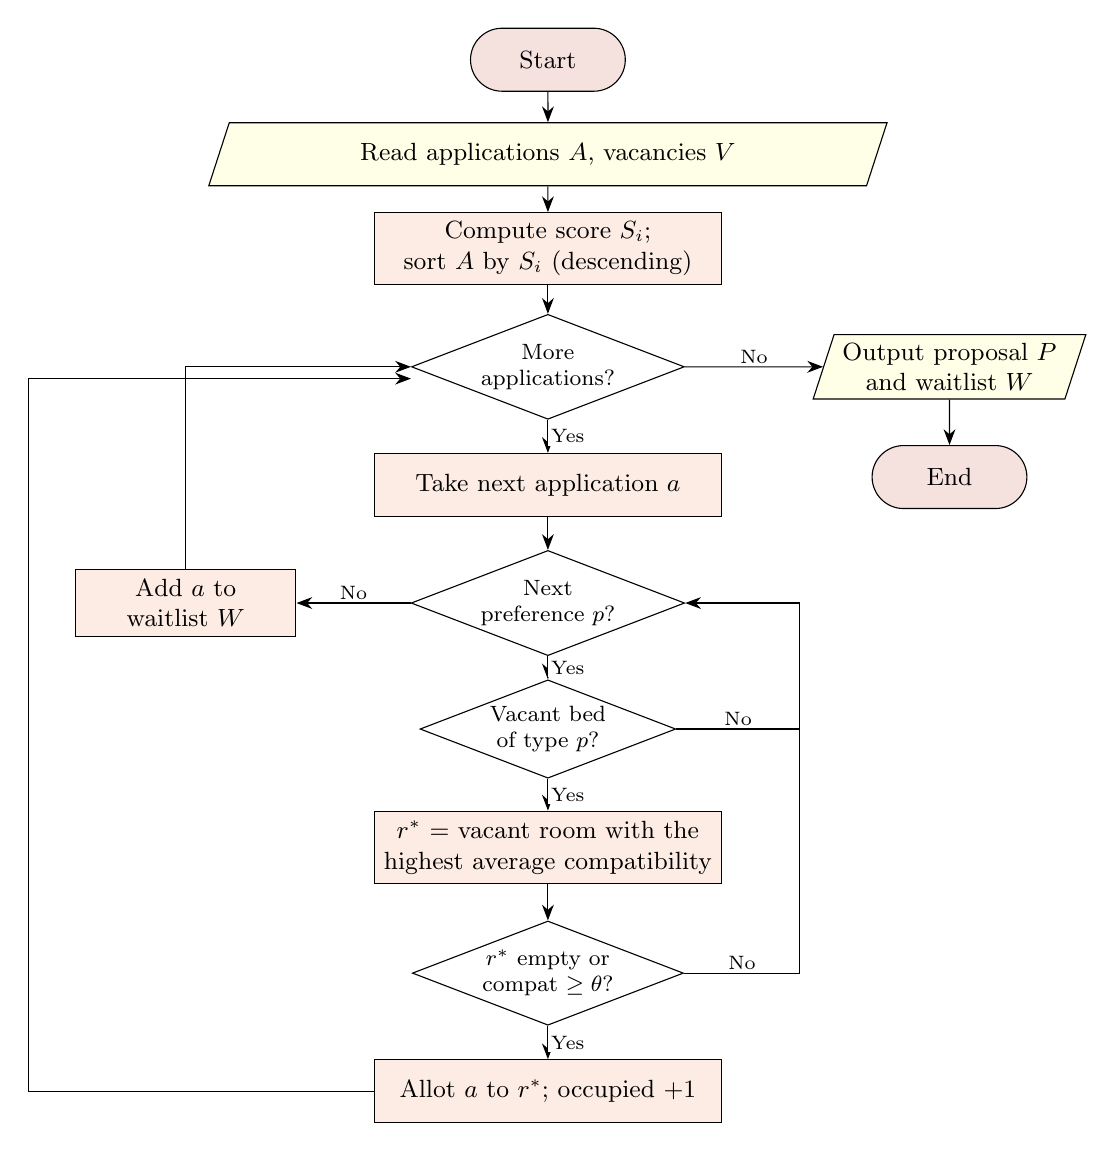
\begin{tikzpicture}[font=\small,
 term/.style={draw,rounded rectangle,fill=cgu!15,minimum height=8mm,minimum width=22mm},
 io/.style={draw,trapezium,trapezium left angle=72,trapezium right angle=108,fill=yellow!10,minimum height=8mm,align=center,inner sep=3pt},
 pr/.style={draw,fill=soft,minimum height=8mm,minimum width=44mm,align=center},
 dc/.style={draw,diamond,aspect=2.6,fill=white,align=center,inner sep=1pt,font=\footnotesize},
 a/.style={-{Stealth[length=2mm]}},yl/.style={font=\scriptsize,fill=white,inner sep=1pt}]
\node[term] (st) at (0,0) {Start};
\node[io] (in) at (0,-1.2) {Read applications $A$, vacancies $V$};
\node[pr] (so) at (0,-2.4) {Compute score $S_i$;\\ sort $A$ by $S_i$ (descending)};
\node[dc] (ma) at (0,-3.9) {More\\applications?};
\node[io] (out) at (5.1,-3.9) {Output proposal $P$\\and waitlist $W$};
\node[term] (en) at (5.1,-5.3) {End};
\node[pr] (tk) at (0,-5.4) {Take next application $a$};
\node[dc] (mp) at (0,-6.9) {Next\\preference $p$?};
\node[pr,minimum width=28mm] (wl) at (-4.6,-6.9) {Add $a$ to\\waitlist $W$};
\node[dc] (vc) at (0,-8.5) {Vacant bed\\of type $p$?};
\node[pr] (pk) at (0,-10.0) {$r^*$ = vacant room with the\\highest average compatibility};
\node[dc] (cp) at (0,-11.6) {$r^*$ empty or\\compat $\ge \theta$?};
\node[pr] (al) at (0,-13.1) {Allot $a$ to $r^*$; occupied $+1$};
\draw[a] (st)--(in); \draw[a] (in)--(so); \draw[a] (so)--(ma);
\draw[a] (ma)--node[yl,above]{No}(out); \draw[a] (out)--(en);
\draw[a] (ma)--node[yl,right]{Yes}(tk); \draw[a] (tk)--(mp);
\draw[a] (mp)--node[yl,above]{No}(wl); \draw[a] (wl.north)|-(ma.west);
\draw[a] (mp)--node[yl,right]{Yes}(vc); \draw[a] (vc)--node[yl,right]{Yes}(pk); \draw[a] (pk)--(cp);
\draw[a] (cp)--node[yl,right]{Yes}(al);
\draw (vc.east)--node[yl,above]{No}(3.2,-8.5);
\draw[a] (cp.east)--node[yl,above]{No}(3.2,-11.6)--(3.2,-6.9)--(mp.east);
\draw[a] (al.west)--(-6.6,-13.1)|-([yshift=-1.5mm]ma.west);
\end{tikzpicture}
\caption{Flowchart of the smart allotment algorithm}\label{fig:flowchart}
\end{figure}

\paragraph{Complexity.} Sorting takes $O(n \log n)$ for $n$ applications. Each application checks at most 3 preferences and, for each, scans the vacant rooms of that type ($m$ at most) with a compatibility check against at most 2 occupants. The total is $O(n \log n + 3nm)$. For 1,000 applications and 400 rooms that is well under a million basic operations, which comfortably meets the 10-second target in NFR1.

\paragraph{Concurrency.} Waitlist promotions can run while a warden is publishing. The \texttt{room} row carries a \texttt{version} column; an allotment commits only if \texttt{UPDATE room SET occupied = occupied + 1, version = version + 1 WHERE room\_id = ? AND version = ? AND occupied < capacity} affects exactly one row. Otherwise the transaction rolls back and retries with fresh data. This makes over-allotment impossible even under concurrent writes.

\paragraph{Fairness and override.} The warden may override any proposal, but must enter a reason. Overrides are logged and appear in a monthly report to the chief warden, so the rule stays the default and exceptions stay visible.

\section{Roommate Compatibility}\label{sec:compat}
Room disputes are one of the most common complaints wardens handle. SHMC reduces them by matching lifestyle habits. Each student answers five questions on a 1--5 scale.

\begin{table}[H]
\centering\small
\caption{Lifestyle survey dimensions}\label{tab:survey}
\begin{tabularx}{\textwidth}{clLc}
\toprule
$k$ & \textbf{Dimension} & \textbf{Scale (1 \ldots 5)} & $w_k$\\
\midrule
1 & Sleep time & before 10 pm \ldots\ after 2 am & 2.0\\
2 & Night study & never \ldots\ every night & 1.5\\
3 & Cleanliness & relaxed \ldots\ very tidy & 1.5\\
4 & Noise tolerance & need silence \ldots\ fine with noise & 1.0\\
5 & Guests & rarely \ldots\ very often & 1.0\\
\bottomrule
\end{tabularx}
\end{table}

Compatibility between students $a$ and $b$ is one minus their weighted distance, scaled by the largest possible distance (4 points on each dimension):
\begin{equation}
\text{compat}(a,b) = 1 - \frac{\sum_{k=1}^{5} w_k \,|a_k - b_k|}{4\sum_{k=1}^{5} w_k}
\end{equation}

\paragraph{Example.} Let $a = (2,4,5,3,2)$, $b = (3,4,4,3,1)$ and $c = (5,1,2,1,5)$. Then $\sum w_k|a_k-b_k| = 2(1)+1.5(0)+1.5(1)+1(0)+1(1) = 4.5$, so $\text{compat}(a,b) = 1 - 4.5/28 = 0.84$. For $a$ and $c$ the distance is 20, giving $0.29$. With the default threshold $\theta = 0.6$, $a$ can share with $b$ but the engine will not place $a$ with $c$ unless no other room is free.

\section{Tamper-Proof QR Gate Pass}\label{sec:qr}
\subsection{Design}
When a leave request is approved, the Gate Pass service issues a token of the form
\[
\text{token} = \underbrace{\text{base64url}(\text{payload})}_{\text{readable}} \;\|\; \text{``.''} \;\|\; \underbrace{\text{base64url}\big(\text{HMAC-SHA256}(K, \text{payload})\big)}_{\text{signature}}
\]
where the payload is a small JSON object: \texttt{\{kid, leaveId, rollNo, validFrom, validTo, nonce\}}. $K$ is a 256-bit secret known only to the server and, in encrypted form, to the guard devices. The token is rendered as a QR code in the student's app.

\subsection{Verification at the Gate}
The guard's scanner verifies a pass in four checks, all of which work without network access:
\begin{enumerate}
  \item Recompute the HMAC over the payload with key \texttt{kid} and compare in constant time.
  \item Check that the current time lies inside $[\text{validFrom}, \text{validTo}]$ for exit, or up to 24 hours after \texttt{validTo} for a (late) return.
  \item Check the local log that this \texttt{nonce} has not already been used in the same direction.
  \item Show the student's photo from the local cache so the guard can match the face.
\end{enumerate}
Scans are queued locally and synced when the network returns; the server then flags late returns to the warden.

\begin{figure}[!htbp]
\centering
\resizebox{0.92\textwidth}{!}{%
\begin{sequencediagram}
\newthread{w}{:Warden}
\newinst[1.3]{gp}{:GatePassService}
\newinst[1.3]{st}{:StudentApp}
\newinst[1.3]{gd}{:GuardScanner}
\begin{call}{w}{approve(leaveId)}{gp}{ok}
  \begin{callself}{gp}{sign payload with K}{token}\end{callself}
\end{call}
\mess{gp}{push QR token}{st}
\begin{call}{gd}{scan QR}{st}{token}\end{call}
\begin{callself}{gd}{verify HMAC, time, nonce}{valid}\end{callself}
\mess{gd}{sync scan log, when online}{gp}
\end{sequencediagram}}
\caption{Sequence diagram: issuing and scanning a QR gate pass}\label{fig:seqqr}
\end{figure}

\subsection{Threat Analysis}
\begin{table}[H]
\centering\small
\caption{Threats to the gate pass and mitigations}\label{tab:qrthreat}
\begin{tabularx}{\textwidth}{lL}
\toprule
\textbf{Threat} & \textbf{Mitigation}\\
\midrule
Student edits dates in the payload & Signature check fails; any change to the payload changes the HMAC\\
Forged pass from scratch & Impossible without $K$; HMAC-SHA256 has no known practical forgery\\
Screenshot shared with a friend & Photo match by the guard; nonce is single-use per direction\\
Replay of an old pass & Time window check plus nonce log\\
Stolen guard phone & $K$ is stored encrypted and bound to the device; keys rotate each semester using \texttt{kid}\\
\bottomrule
\end{tabularx}
\end{table}

\section{SLA-Based Complaint Escalation}
Every complaint category has a maximum resolution time. The deadline is set when the complaint is raised: $\text{deadline} = \text{raisedAt} + \text{SLA}(\text{category})$.

\begin{table}[H]
\centering\small
\caption{Service levels by complaint category}\label{tab:sla}
\begin{tabular}{lcl}
\toprule
\textbf{Category} & \textbf{SLA (hours)} & \textbf{Escalates to}\\
\midrule
Electrical (no power, sparking) & 12 & Chief warden and estate office\\
Plumbing (leak, no water) & 24 & Chief warden\\
Cleaning & 24 & Chief warden\\
Furniture and fittings & 72 & Chief warden\\
Internet / Wi-Fi & 48 & Chief warden and IT cell\\
Other & 72 & Chief warden\\
\bottomrule
\end{tabular}
\end{table}

A scheduled job runs every 15 minutes and selects complaints where \texttt{status IN ('OPEN','ASSIGNED','IN\_PROGRESS') AND sla\_deadline < NOW() AND escalated = 0}. Each one moves to \emph{Escalated}, and the chief warden is notified. The warden dashboard shows the SLA compliance rate, defined as the share of complaints resolved before their deadline over the last 30 days. This single number gives the administration a way to measure maintenance quality that simply does not exist today.

\section{Occupancy Forecasting}\label{sec:forecast}
Halls are planned a year ahead, but today nobody estimates demand from data. SHMC fits a least-squares line to past application counts for each hall and projects one session forward:
\begin{equation}
\hat{y} = \beta_0 + \beta_1 x, \qquad \beta_1 = \frac{\sum (x_i-\bar x)(y_i-\bar y)}{\sum (x_i-\bar x)^2}, \qquad \beta_0 = \bar y - \beta_1 \bar x
\end{equation}

\paragraph{Illustration.} Suppose a hall received 410, 438, 455, 490 and 512 applications in the five sessions from 2021-22 to 2025-26 ($x = 1 \ldots 5$). Then $\beta_1 = 25.6$ and $\beta_0 = 384.2$, with $R^2 = 0.99$. The forecast for 2026-27 ($x=6$) is $\hat{y} = 384.2 + 25.6 \times 6 \approx 538$ applications. If the hall has 520 beds, the dashboard shows a projected shortfall of 18 beds before the session begins, early enough to reassign capacity.

\begin{figure}[!htbp]
\centering
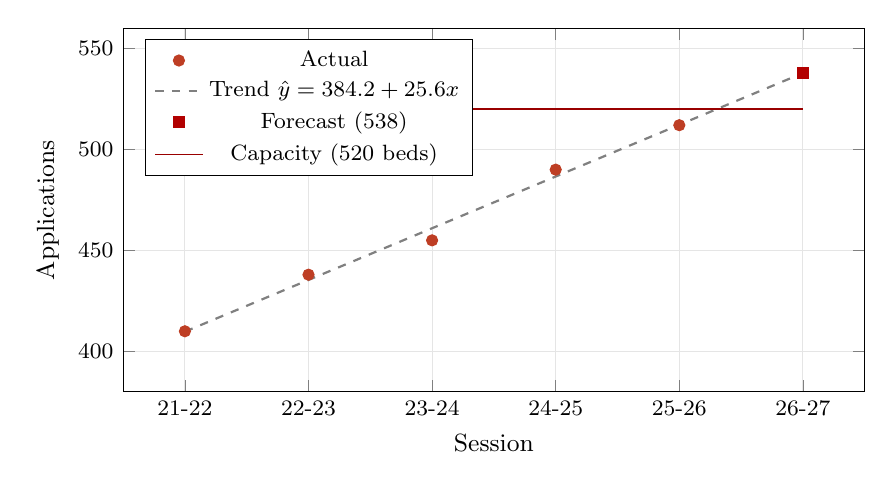
\begin{tikzpicture}
\begin{axis}[width=11cm,height=6.2cm,xlabel={Session},ylabel={Applications},
  xtick={1,...,6},xticklabels={21-22,22-23,23-24,24-25,25-26,26-27},
  ymin=380,ymax=560,grid=major,grid style={gray!20},legend pos=north west,legend style={font=\footnotesize},
  tick label style={font=\footnotesize},label style={font=\small}]
\addplot[only marks,mark=*,cgu] coordinates {(1,410)(2,438)(3,455)(4,490)(5,512)};
\addlegendentry{Actual}
\addplot[domain=1:6,dashed,thick,gray] {384.2+25.6*x};
\addlegendentry{Trend $\hat y = 384.2 + 25.6x$}
\addplot[only marks,mark=square*,red!70!black] coordinates {(6,538)};
\addlegendentry{Forecast (538)}
\addplot[domain=1:6,thin,red!60!black] {520};
\addlegendentry{Capacity (520 beds)}
\end{axis}
\end{tikzpicture}
\caption{Illustrative demand forecast for one hall}\label{fig:forecast}
\end{figure}

A straight line is deliberately simple. With only five data points per hall, a more complex model would overfit. The module is designed so that the model can be swapped later, once more years of data exist.

%================ CHAPTER 9 =================
\chapter{API and Security Design}

\section{REST API}
All endpoints live under \texttt{/api/v1}, accept and return JSON, and require a bearer JWT except where marked public.

\begin{longtable}{p{1.3cm}p{5.4cm}p{2.6cm}p{5.2cm}}
\caption{Main API endpoints}\label{tab:api}\\
\toprule
\textbf{Method} & \textbf{Endpoint} & \textbf{Role} & \textbf{Purpose}\\
\midrule\endfirsthead
\toprule
\textbf{Method} & \textbf{Endpoint} & \textbf{Role} & \textbf{Purpose}\\
\midrule\endhead
POST & /auth/login & public & Returns access and refresh tokens\\
POST & /auth/refresh & public & Rotates refresh token, issues new access token\\
GET & /halls/\{id\}/vacancies & warden, student & Vacancy by type and floor\\
POST & /applications & student & Submit room application\\
POST & /halls/\{id\}/allotment/run & warden & Run engine, return proposal\\
POST & /halls/\{id\}/allotment/publish & warden & Publish proposal\\
POST & /transfers & student & Request room transfer\\
GET & /invoices?status=unpaid & student, accountant & List invoices\\
POST & /payments/order & student & Create gateway order\\
POST & /payments/webhook & gateway (HMAC) & Payment status callback\\
POST & /complaints & student & Raise complaint (multipart with photo)\\
PATCH & /complaints/\{id\} & warden, staff & Assign or change status\\
POST & /leaves & student & Apply for leave\\
PATCH & /leaves/\{id\}/approve & warden & Approve and issue QR pass\\
POST & /gate/scans & guard & Upload batched scan log\\
POST & /visitors & guard & Record visitor entry\\
GET & /analytics/forecast & warden, admin & Demand forecast per hall\\
\bottomrule
\end{longtable}

\section{Authentication Flow}
On login the server checks the bcrypt hash and returns a short-lived \textbf{access token} (JWT, 15 minutes, signed with RS256) and a long-lived \textbf{refresh token} (random 256-bit string, 7 days, stored hashed in Redis). The access token carries \texttt{sub}, \texttt{role} and \texttt{hallId}. When it expires, the client calls \texttt{/auth/refresh}; the old refresh token is revoked and a new pair is issued. Reuse of a revoked refresh token signals theft, so all of that user's sessions are cut.

\section{Role-Based Access Control}
\begin{table}[H]
\centering\small
\caption{RBAC permission matrix}\label{tab:rbac}
\begin{tabular}{lcccccc}
\toprule
\textbf{Permission} & \textbf{Student} & \textbf{Warden} & \textbf{Chief W.} & \textbf{Acct.} & \textbf{Mess} & \textbf{Guard}\\
\midrule
Apply for room & \checkmark & & & & & \\
Run / publish allotment & & \checkmark & \checkmark & & & \\
Pay own invoice & \checkmark & & & & & \\
Define fee heads & & & & \checkmark & & \\
Raise complaint & \checkmark & & & & & \\
Assign complaint & & \checkmark & \checkmark & & & \\
Approve leave & & \checkmark & \checkmark & & & \\
Scan gate pass & & & & & & \checkmark\\
Update mess menu & & & & & \checkmark & \\
View analytics & & \checkmark & \checkmark & \checkmark & & \\
\bottomrule
\end{tabular}
\end{table}

Permissions are checked on the server for every request. A warden's token also carries \texttt{hallId}, and every query is filtered by it, so a warden cannot read another hall's data even by editing a URL.

\section{Mapping to OWASP Top 10}
\begin{table}[H]
\centering\small
\caption{Security controls against common web risks}\label{tab:owasp}
\begin{tabularx}{\textwidth}{lL}
\toprule
\textbf{Risk} & \textbf{Control in SHMC}\\
\midrule
Broken access control & Server-side RBAC plus hall scoping on every query\\
Cryptographic failures & TLS 1.2+, bcrypt cost 12, RS256 JWTs, HMAC-SHA256 gate passes\\
Injection & Parameterised queries only; JSON-schema validation on all inputs\\
Insecure design & Payment state set only from signed webhooks; idempotent webhook handling via unique \texttt{gateway\_ref}\\
Security misconfiguration & Helmet security headers; secrets in environment variables, never in Git\\
Vulnerable components & \texttt{npm audit} in CI; Dependabot updates\\
Authentication failures & Lockout after 5 attempts; refresh-token rotation with reuse detection\\
Logging failures & Audit table for allotment, payment and complaint changes (NFR10)\\
\bottomrule
\end{tabularx}
\end{table}
%================ CHAPTER 10 =================
\chapter{Size, Effort and Schedule Estimation}
We estimate size bottom-up with Function Point Analysis, convert it to lines of code, and then derive effort and schedule with Intermediate COCOMO.

\section{Function Point Analysis}
\subsection{Counting the Functions}
Table~\ref{tab:fpcount} counts the five function types from the SRS and assigns each a complexity using the standard IFPUG weights.

\begin{table}[H]
\centering\small
\caption{Unadjusted function point count}\label{tab:fpcount}
\begin{tabular}{lccccc}
\toprule
\textbf{Function type} & \textbf{Simple} & \textbf{Average} & \textbf{Complex} & \textbf{Examples} & \textbf{UFP}\\
\midrule
External Inputs (EI) & $5\times3$ & $7\times4$ & $2\times6$ & application, payment, complaint & 55\\
External Outputs (EO) & $2\times4$ & $4\times5$ & $2\times7$ & receipt, reports, QR pass & 42\\
External Inquiries (EQ) & $3\times3$ & $3\times4$ & $0\times6$ & vacancy, status, history & 21\\
Internal Logical Files (ILF) & $6\times7$ & $4\times10$ & $1\times15$ & student, room, allotment & 97\\
External Interface Files (EIF) & $2\times5$ & $1\times7$ & $0\times10$ & gateway, SMS, enrolment CSV & 17\\
\midrule
\multicolumn{5}{r}{\textbf{Total unadjusted function points (UFP)}} & \textbf{232}\\
\bottomrule
\end{tabular}
\end{table}

\subsection{Value Adjustment Factor}
The fourteen general system characteristics are rated from 0 (no influence) to 5 (essential).

\begin{table}[H]
\centering\small
\caption{General system characteristics}\label{tab:gsc}
\begin{tabular}{llc@{\hspace{1.2cm}}llc}
\toprule
\textbf{\#} & \textbf{Characteristic} & $\mathbf{F_i}$ & \textbf{\#} & \textbf{Characteristic} & $\mathbf{F_i}$\\
\midrule
1 & Data communications & 4 & 8 & Online update & 4\\
2 & Distributed data processing & 2 & 9 & Complex processing & 3\\
3 & Performance & 4 & 10 & Reusability & 2\\
4 & Heavily used configuration & 3 & 11 & Installation ease & 2\\
5 & Transaction rate & 4 & 12 & Operational ease & 3\\
6 & Online data entry & 5 & 13 & Multiple sites & 1\\
7 & End-user efficiency & 4 & 14 & Facilitate change & 1\\
\midrule
\multicolumn{5}{r}{$\sum F_i$} & \textbf{42}\\
\bottomrule
\end{tabular}
\end{table}

\begin{align*}
\text{VAF} &= 0.65 + 0.01 \sum F_i = 0.65 + 0.42 = 1.07\\
\text{FP} &= \text{UFP} \times \text{VAF} = 232 \times 1.07 = 248.2 \approx 248
\end{align*}

\subsection{Conversion to Lines of Code}
Using an industry average of about 47 lines of JavaScript per function point:
\[
\text{Size} = 248 \times 47 \approx 11{,}656 \text{ LOC} \approx 11.7 \text{ KLOC}
\]

\section{COCOMO Estimation}\label{sec:cocomo}
\subsection{Project Mode}
SHMC is an \textbf{organic} project: a small team working in a familiar domain with well-understood requirements and few hard constraints. The organic constants are $a = 3.2$ and $b = 1.05$ for Intermediate COCOMO (2.4 for Basic), with $c = 2.5$ and $d = 0.38$ for schedule.

\subsection{Basic COCOMO (for comparison)}
\[
E_{\text{basic}} = 2.4 \times (11.7)^{1.05} = 31.8 \text{ person-months}
\]

\subsection{Intermediate COCOMO}
Basic COCOMO ignores the team and the product. Intermediate COCOMO corrects the nominal effort with fifteen cost drivers. Our ratings are in Table~\ref{tab:drivers}.

\begin{table}[H]
\centering\small
\caption{Cost driver ratings}\label{tab:drivers}
\begin{tabularx}{\textwidth}{llcL}
\toprule
\textbf{Driver} & \textbf{Rating} & \textbf{Multiplier} & \textbf{Reason}\\
\midrule
RELY Required reliability & High & 1.15 & Money and allotment data must be correct\\
DATA Database size & Nominal & 1.00 & Tens of thousands of rows\\
CPLX Product complexity & High & 1.15 & Allotment engine, HMAC, concurrency\\
TIME Execution time constraint & Nominal & 1.00 & \\
STOR Storage constraint & Nominal & 1.00 & \\
VIRT Platform volatility & Low & 0.87 & Stable LTS stack\\
TURN Turnaround time & Low & 0.87 & Local dev with hot reload\\
ACAP Analyst capability & High & 0.86 & Team did detailed analysis (this report)\\
AEXP Application experience & Nominal & 1.00 & Team are hostel residents themselves\\
PCAP Programmer capability & High & 0.86 & \\
VEXP Platform experience & Nominal & 1.00 & \\
LEXP Language experience & High & 0.95 & JavaScript used across coursework\\
MODP Modern practices & High & 0.91 & Git, code review, CI\\
TOOL Software tools & High & 0.91 & Mature IDE, linters, test runners\\
SCED Schedule constraint & Nominal & 1.00 & \\
\midrule
\multicolumn{2}{r}{\textbf{EAF (product)}} & \textbf{0.582} & \\
\bottomrule
\end{tabularx}
\end{table}

\begin{align*}
E_{\text{nom}} &= 3.2 \times (11.7)^{1.05} = 42.3 \text{ PM}\\
E &= E_{\text{nom}} \times \text{EAF} = 42.3 \times 0.582 = 24.7 \text{ person-months}\\
T_{\text{dev}} &= 2.5 \times E^{0.38} = 2.5 \times 24.7^{0.38} = 8.5 \text{ months}\\
\text{Staff} &= E / T_{\text{dev}} = 24.7 / 8.5 \approx 2.9 \approx 3 \text{ persons}\\
\text{Cost} &= 24.7 \times \text{Rs. } 40{,}000 \approx \text{Rs. } 9.9 \text{ lakh}
\end{align*}

The estimate of about three people for eight and a half months matches our actual team and two academic semesters. The cost figure assumes a market rate of Rs.~40,000 per person-month for a junior developer.

\section{Project Schedule}
Figure~\ref{fig:gantt} lays the three increments over 36 weeks. Testing of each increment overlaps the start of the next, which is how the incremental model saves calendar time.

\begin{figure}[!htbp]
\centering
\resizebox{\textwidth}{!}{%
\begin{ganttchart}[hgrid,vgrid={*3{draw=none},dotted},x unit=0.42cm,y unit chart=0.62cm,
  bar/.append style={fill=cgu!45},bar height=0.55,group/.append style={fill=cgu},
  milestone/.append style={fill=red!70!black},title label font=\scriptsize,bar label font=\small,milestone label font=\small\itshape]{1}{36}
\gantttitle{Weeks}{36}\\
\gantttitlelist{1,...,36}{1}\\
\ganttbar{Requirements and SRS}{1}{3}\\
\ganttbar{Architecture and design}{3}{7}\\
\ganttgroup{Increment 1}{7}{15}\\
\ganttbar{Develop I1}{7}{13}\\
\ganttbar{Test I1}{12}{15}\\
\ganttmilestone{I1 live (allotment)}{15}\\
\ganttgroup{Increment 2}{15}{23}\\
\ganttbar{Develop I2}{15}{21}\\
\ganttbar{Test I2}{20}{23}\\
\ganttmilestone{I2 live (fees, mess)}{23}\\
\ganttgroup{Increment 3}{23}{33}\\
\ganttbar{Develop I3}{23}{30}\\
\ganttbar{Test I3}{29}{33}\\
\ganttbar{Deployment and acceptance}{33}{36}\\
\ganttmilestone{Handover}{36}
\end{ganttchart}}
\caption{Project schedule (Gantt chart)}\label{fig:gantt}
\end{figure}

\section{Team Organisation}
\begin{table}[H]
\centering\small
\caption{Roles and responsibilities}\label{tab:team}
\begin{tabularx}{\textwidth}{lL}
\toprule
\textbf{Member} & \textbf{Primary responsibilities}\\
\midrule
Sk Mustakim Ali & Backend lead: API, allotment engine, database design, deployment\\
Suprit Kumar Naik & Frontend lead: React PWA, guard scanner, dashboards and charts\\
Sweta Samantaray & Quality and integration: test plan, payment and notification integration, documentation\\
\bottomrule
\end{tabularx}
\end{table}
All three members review each other's pull requests, and each module is known by at least two people, which also mitigates the personnel risk in Chapter~12.

%================ CHAPTER 11 =================
\chapter{Testing}

\section{Test Strategy}
Testing follows the V-model mapping inside each increment: unit tests check the design of individual functions, integration tests check module interfaces, system tests check the SRS, and acceptance tests check that users can actually do their jobs.

\begin{table}[H]
\centering\small
\caption{Levels of testing}\label{tab:levels}
\begin{tabularx}{\textwidth}{llL}
\toprule
\textbf{Level} & \textbf{Tool} & \textbf{Focus}\\
\midrule
Unit & Jest & Score formula, compatibility, fine calculation, HMAC sign/verify, state transitions\\
Integration & Jest + Supertest, test MySQL & API to database; allotment updating rooms and raising invoices; webhook to receipt\\
System & Playwright, k6 & End-to-end flows per SRS; load test at 500 virtual users\\
Security & OWASP ZAP & Injection, broken access control, header checks\\
Acceptance & Real users & One warden and 20 students use the system for a week in parallel with paper\\
\bottomrule
\end{tabularx}
\end{table}

\section{White-Box Testing of the Allotment Algorithm}
\subsection{Flow Graph}
Figure~\ref{fig:flowgraph} is the control flow graph of Algorithm~\ref{alg:allot}. Nodes are numbered as follows: 1 sort; 2 more applications?; 3 reset flag; 4 more preferences and not allotted?; 5 vacancy of this type?; 6 compatible?; 7 allot; 8 next preference; 9 allotted?; 10 waitlist; 11 next application; 12 return.

\begin{figure}[!htbp]
\centering
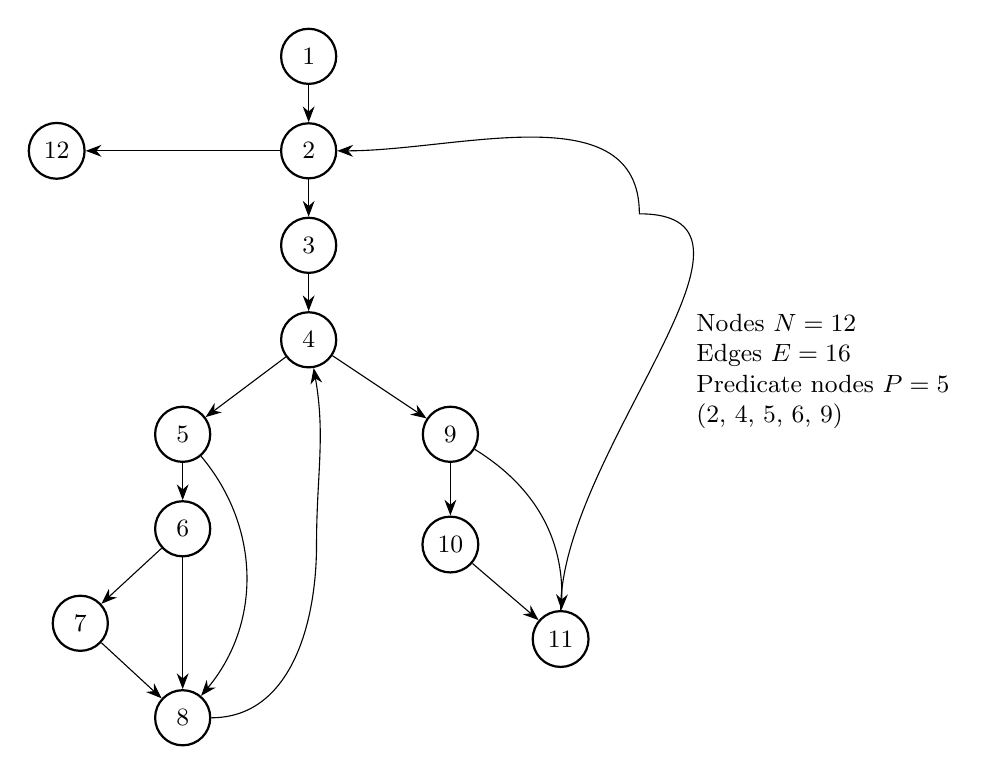
\begin{tikzpicture}[n/.style={circle,draw,thick,minimum size=7mm,font=\small},a/.style={-{Stealth[length=2mm]}}]
\node[n] (1) at (0,0) {1};
\node[n] (2) at (0,-1.2) {2};
\node[n] (3) at (0,-2.4) {3};
\node[n] (4) at (0,-3.6) {4};
\node[n] (5) at (-1.6,-4.8) {5};
\node[n] (6) at (-1.6,-6.0) {6};
\node[n] (7) at (-2.9,-7.2) {7};
\node[n] (8) at (-1.6,-8.4) {8};
\node[n] (9) at (1.8,-4.8) {9};
\node[n] (10) at (1.8,-6.2) {10};
\node[n] (11) at (3.2,-7.4) {11};
\node[n] (12) at (-3.2,-1.2) {12};
\draw[a] (1)--(2); \draw[a] (2)--(3); \draw[a] (2)--(12); \draw[a] (3)--(4);
\draw[a] (4)--(5); \draw[a] (4)--(9); \draw[a] (5)--(6);
\draw[a] (5) to[bend left=40] (8);
\draw[a] (6)--(7); \draw[a] (6)--(8); \draw[a] (7)--(8);
\draw[a] (8) to[out=0,in=-90] (0.1,-6.2) to[out=90,in=-80] (4);
\draw[a] (9)--(10); \draw[a] (9) to[bend left=30] (11); \draw[a] (10)--(11);
\draw[a] (11) to[out=90,in=0] (4.2,-2) to[out=90,in=0] (2);
\node[font=\small,align=left,anchor=west] at (4.8,-4) {Nodes $N = 12$\\Edges $E = 16$\\Predicate nodes $P = 5$\\(2, 4, 5, 6, 9)};
\end{tikzpicture}
\caption{Control flow graph (program graph) of the allotment algorithm}\label{fig:flowgraph}
\end{figure}

\subsection{Cyclomatic Complexity}
All three standard formulas agree:
\[
V(G) = E - N + 2 = 16 - 12 + 2 = 6, \qquad V(G) = P + 1 = 5 + 1 = 6, \qquad V(G) = \text{number of regions} = 6
\]
So at least six test cases are needed to exercise every independent path. A value of 6 also sits comfortably below the common threshold of 10, which suggests the function does not need to be split further.

\subsection{Basis Paths and Test Cases}
\begin{table}[H]
\centering\small
\caption{Basis paths with test data}\label{tab:basis}
\begin{tabularx}{\textwidth}{clLL}
\toprule
\textbf{\#} & \textbf{Path} & \textbf{Input} & \textbf{Expected}\\
\midrule
1 & 1-2-12 & No applications & Empty proposal and waitlist\\
2 & 1-2-3-4-9-10-11-2-12 & One application with an empty preference list & Student waitlisted\\
3 & 1-2-3-4-5-8-4-9-10-11-2-12 & One application; no vacancy in any preferred type & Student waitlisted\\
4 & 1-2-3-4-5-6-8-4-9-10-11-2-12 & Only vacancy is with an occupant of compatibility 0.29 & Student waitlisted\\
5 & 1-2-3-4-5-6-7-8-4-9-11-2-12 & Empty double room available & Student allotted to it\\
6 & 1-2-3-4-5-6-7-8-4-9-11-2-3-4-5-8-4-9-10-11-2-12 & Two applications, one bed & Higher score allotted; other waitlisted\\
\bottomrule
\end{tabularx}
\end{table}

\section{Black-Box Testing}
\subsection{Equivalence Partitioning and Boundary Values}
\begin{table}[H]
\centering\small
\caption{Equivalence classes and boundary values}\label{tab:ecp}
\begin{tabularx}{\textwidth}{lLLL}
\toprule
\textbf{Input} & \textbf{Valid class} & \textbf{Invalid classes} & \textbf{Boundary values tested}\\
\midrule
CGPA & $0.00 \le x \le 10.00$ & $x < 0$; $x > 10$; non-numeric & $-0.01, 0.00, 0.01, 9.99, 10.00, 10.01$\\
Leave duration & 1--30 days, start $\ge$ today & end before start; $> 30$ days; start in the past & 0, 1, 30, 31 days\\
Room occupancy & $0 \le$ occupied $\le$ capacity & occupied $>$ capacity & capacity $-1$, capacity, capacity $+1$\\
Payment amount & equals invoice balance & less; more; negative & balance $\pm$ Rs.~1\\
Password & 8--64 chars, 1 digit, 1 letter & too short; too long; no digit & 7, 8, 64, 65 chars\\
\bottomrule
\end{tabularx}
\end{table}

\subsection{System Test Cases}
\begin{longtable}{p{0.9cm}p{2.1cm}p{5.6cm}p{5.6cm}}
\caption{Selected system test cases}\label{tab:tc}\\
\toprule
\textbf{ID} & \textbf{Module} & \textbf{Steps / input} & \textbf{Expected result}\\
\midrule\endfirsthead
\toprule
\textbf{ID} & \textbf{Module} & \textbf{Steps / input} & \textbf{Expected result}\\
\midrule\endhead
TC01 & Login & Valid roll number and password & Dashboard for the user's role opens\\
TC02 & Login & Wrong password 5 times in a row & Account locked for 15 minutes; email sent\\
TC03 & Login & Student token calls a warden-only endpoint & HTTP 403; attempt logged\\
TC04 & Application & Submit with pending dues & Blocked with link to invoice\\
TC05 & Application & Choose a hall of the other gender & Option not shown; API returns 422 if forced\\
TC06 & Allotment & Run engine on 1,000 test applications & Completes in under 10 s; no room over capacity\\
TC07 & Allotment & Two wardens publish the same room at once & One commit succeeds; other retries with fresh data\\
TC08 & Allotment & Warden overrides without a reason & Save disabled; reason is mandatory\\
TC09 & Payment & Gateway webhook with valid signature & Invoice PAID; receipt PDF emailed\\
TC10 & Payment & Webhook with tampered amount & Signature check fails; invoice unchanged\\
TC11 & Payment & Same webhook delivered twice & Second call ignored (unique gateway\_ref)\\
TC12 & Payment & Payment one day after due date & Late fine added to the invoice\\
TC13 & Complaint & Raise electrical complaint, leave it 13 h & Status Escalated; chief warden notified\\
TC14 & Complaint & Student reopens after 49 h & Rejected; complaint already auto-closed\\
TC15 & Gate pass & Scan a valid pass during leave window & Green result with photo; exit time logged\\
TC16 & Gate pass & Payload date edited by hand & Red result: invalid signature\\
TC17 & Gate pass & Same QR scanned twice for exit & Second scan rejected: already used\\
TC18 & Gate pass & Scanner offline during scan & Verified locally; synced when online\\
TC19 & Visitor & Visitor entry at 8:30 pm & Blocked with message about visiting hours\\
TC20 & Forecast & Five sessions of sample data & Forecast 538 for sample hall (Section~\ref{sec:forecast})\\
\bottomrule
\end{longtable}

\section{Non-Functional Testing}
\textbf{Load.} A k6 script ramps to 500 virtual users over two minutes and holds for ten, mixing vacancy lookups, application submissions and dashboard loads. Pass criterion: p95 latency under 500 ms and error rate under 0.5\%.

\textbf{Security.} OWASP ZAP runs a baseline scan in CI on every merge to the main branch. Any high-severity alert fails the build.

\textbf{Usability.} Five first-year students who have never seen the system are asked to apply for a room. Success means all five finish in under five minutes without help (NFR6). An increment is released when all Must-have requirements in its scope pass, unit coverage on service code is at least 80\%, there are no open critical or high defects, and the load test passes.
%================ CHAPTER 12 =================
\chapter{Risk Management}

\section{Risk Identification and Analysis}
Each risk is rated for probability (1 = low, 3 = high) and impact (1 = minor, 4 = critical). Risk exposure is their product, and the table is sorted by it.

\begin{table}[H]
\centering\small
\caption{Risk register}\label{tab:risk}
\begin{tabularx}{\textwidth}{clccc}
\toprule
\textbf{ID} & \textbf{Risk} & \textbf{P} & \textbf{I} & \textbf{Exposure}\\
\midrule
R1 & Server overload during semester-start allotment & 3 & 4 & 12\\
R2 & Low adoption by wardens used to registers & 2 & 4 & 8\\
R3 & Payment gateway failure or duplicate charge & 2 & 3 & 6\\
R4 & Hall rules change mid-project & 3 & 2 & 6\\
R5 & Team member unavailable (exams, illness) & 2 & 3 & 6\\
R6 & Breach of student personal data & 1 & 4 & 4\\
R7 & Gate-pass signing key leaked & 1 & 4 & 4\\
R8 & Schedule overrun of Increment 3 & 2 & 2 & 4\\
\bottomrule
\end{tabularx}
\end{table}

\section{RMMM Plan}
{\footnotesize
\begin{longtable}{p{0.8cm}p{4.6cm}p{4.3cm}p{4.3cm}}
\caption{Risk mitigation, monitoring and management}\label{tab:rmmm}\\
\toprule
\textbf{ID} & \textbf{Mitigation (reduce P or I)} & \textbf{Monitoring (early signal)} & \textbf{Management (if it happens)}\\
\midrule\endfirsthead
\toprule
\textbf{ID} & \textbf{Mitigation} & \textbf{Monitoring} & \textbf{Management}\\
\midrule\endhead
R1 & Load test at 500 users; cache vacancy in Redis; open applications hall by hall over three days & p95 latency and CPU on dashboard; alert at 70\% CPU & Scale VM vertically; queue submissions and confirm by email\\
R2 & Involve two wardens in design reviews; one-hour training; parallel run with paper for two weeks & Weekly count of actions done in SHMC vs on paper & Assign a team member to sit with the hall office for a week\\
R3 & Webhook-only status; idempotency via unique gateway reference & Daily reconciliation report of gateway vs SHMC totals & Manual refund workflow; incident note to affected students\\
R4 & Rules stored as configuration; incremental delivery & Change requests logged per week & Re-plan the next increment's scope, not the current one\\
R5 & Pair on every module; shared documentation & Weekly stand-up attendance & Re-assign using module pairing\\
R6 & RBAC, hall scoping, encryption in transit, audit logs & Failed-access alerts; ZAP scans & Revoke tokens, rotate secrets, inform affected users within 72 hours\\
R7 & Key per semester with \texttt{kid}; encrypted on device & Scans signed with unknown \texttt{kid} & Rotate key; reissue active passes\\
R8 & Cut Could-have items first (forecast, meal rating) & Burn-down chart against plan & Move Could-have items to a maintenance release\\
\bottomrule
\end{longtable}}

%================ CHAPTER 13 =================
\chapter{Quality Assurance and Maintenance}

\section{Software Quality Assurance}
Quality is built in at every stage rather than tested in at the end.
\begin{itemize}
  \item \textbf{Reviews.} The SRS and design were reviewed with the guide. Every pull request needs one approving review before merge.
  \item \textbf{Standards.} ESLint with the Airbnb style guide, Prettier formatting, and conventional commit messages.
  \item \textbf{Continuous integration.} Each push runs lint, unit tests, integration tests against a MySQL container, and a ZAP baseline scan. A red build blocks merging.
\end{itemize}

\begin{table}[H]
\centering\small
\caption{Quality metrics and targets}\label{tab:metrics}
\begin{tabularx}{\textwidth}{lLc}
\toprule
\textbf{Metric} & \textbf{Definition} & \textbf{Target}\\
\midrule
Defect density & Defects found after release per KLOC & $< 1.0$\\
Unit test coverage & Statement coverage of service-layer code & $\ge 80\%$\\
Cyclomatic complexity & Per function & $\le 10$\\
Mean time to repair & Average time from bug report to fix deployed & $< 48$ h\\
SLA compliance & Complaints resolved within SLA (a product metric) & $\ge 90\%$\\
\bottomrule
\end{tabularx}
\end{table}

\section{Configuration Management}
Code lives in a Git repository with a simple branching model: \texttt{main} is always deployable, each feature is developed on a short-lived branch, and releases are tagged with semantic versions (\texttt{v1.0.0} for Increment~1, \texttt{v1.1.0} for Increment~2, and so on). Database changes are versioned migration files, so any environment can be rebuilt to an exact version. Configuration such as score weights and SLA hours is stored in the database and every change is audited.

\section{Maintenance Plan}
\begin{table}[H]
\centering\small
\caption{Planned maintenance activities}\label{tab:maint}
\begin{tabularx}{\textwidth}{lL}
\toprule
\textbf{Type} & \textbf{Examples in SHMC}\\
\midrule
Corrective & Fixing defects reported through an in-app ``Report a problem'' link\\
Adaptive & Updating to new Razorpay API versions; adapting to new university fee rules\\
Perfective & New reports requested by wardens; better roommate survey questions\\
Preventive & Dependency upgrades each semester; refactoring any function whose complexity grows past 10\\
\bottomrule
\end{tabularx}
\end{table}

%================ CHAPTER 14 =================
\chapter{Implementation and Results}
\newcommand{\sframe}[2]{\fcolorbox{gray!45}{white}{\includegraphics[width=#1]{shots/#2}}}
\newcommand{\shotpair}[6]{\begin{figure}[H]\centering\setlength{\fboxsep}{0pt}%
\begin{minipage}[t]{0.485\textwidth}\centering\sframe{0.985\linewidth}{#1}\\[3pt]{\footnotesize (a) #2}\end{minipage}\hfill
\begin{minipage}[t]{0.485\textwidth}\centering\sframe{0.985\linewidth}{#3}\\[3pt]{\footnotesize (b) #4}\end{minipage}
\caption{#5}\label{#6}\end{figure}}
\newcommand{\shotone}[4]{\begin{figure}[H]\centering\setlength{\fboxsep}{0pt}\sframe{#2}{#1}\caption{#3}\label{#4}\end{figure}}

We built a working prototype of SHMC to show that the design in Chapters~7 to~9 holds up in code. The prototype implements every Must-have requirement in the allotment, fees, complaints, leave/gate and visitor modules, plus the warden dashboard. The complete source code is in Appendix~\ref{app:code}, and every screenshot in this chapter was captured from the running application.

\section{Prototype Technology}
The production design (Chapter~7) uses React, MySQL and Redis. For the prototype we kept the same module boundaries, database schema and API, but chose a lighter stack so that anyone can run it with one command and no database server.

\begin{table}[H]
\centering\small
\caption{Prototype stack compared with the production design}\label{tab:stack}
\begin{tabularx}{\textwidth}{lLL}
\toprule
\textbf{Layer} & \textbf{Prototype (implemented)} & \textbf{Production design}\\
\midrule
Front end & Single-page app in plain HTML, CSS and JavaScript & React 18 PWA\\
Back end & Node.js 22, Express 4 & Same\\
Database & SQLite through Node's built-in \texttt{node:sqlite} & MySQL 8 with replica\\
Sessions & HMAC-signed bearer token, 8-hour expiry & RS256 JWT with refresh tokens in Redis\\
Payments & Mock gateway that signs a real HMAC webhook & Razorpay Orders and Webhooks\\
QR codes & \texttt{qrcode} npm package & Same\\
Testing & Node's built-in test runner (\texttt{node:test}) & Jest, Playwright, k6\\
\bottomrule
\end{tabularx}
\end{table}

The whole prototype is about 700 lines of code across eight files, with only two npm dependencies (\texttt{express} and \texttt{qrcode}).

\section{Project Structure and How to Run}
\begin{lstlisting}
shmc-app/
  server.js        REST API: auth, allotment, fees, complaints, leave, gate, visitors
  engine.js        priority score, roommate compatibility, allotment algorithm
  gate.js          HMAC sign/verify for QR passes and sessions; scrypt passwords
  db.js            SQLite schema (10 tables) and demo seed data
  public/          index.html, app.js (single-page UI), style.css, cgu.png
  test/            shmc.test.js (12 automated tests)
\end{lstlisting}

\begin{lstlisting}
npm install          # installs express and qrcode
npm start            # opens on http://localhost:3000
npm test             # runs the 12 automated tests
\end{lstlisting}
Demo logins (password \texttt{pass123}): students \texttt{2301020456}, \texttt{2301020457}, \texttt{2301020459}; warden \texttt{warden1}; accountant \texttt{accounts}; guard \texttt{guard1}. Deleting \texttt{shmc.db} resets the demo data.

\section{Requirements Implemented}
\begin{table}[H]
\centering\small
\caption{Traceability from requirements to code and evidence}\label{tab:trace}
\begin{tabularx}{\textwidth}{lLll}
\toprule
\textbf{Requirements} & \textbf{Implemented behaviour} & \textbf{Code} & \textbf{Evidence}\\
\midrule
FR1.1, FR1.4 & Login, role-based tabs and API guard (HTTP 403 for wrong role) & \texttt{auth()} & Fig.~\ref{fig:ss-login}, test 12\\
FR2.1--FR2.3 & Application with 3 preferences and lifestyle survey; live priority score & \texttt{score}, \texttt{rank} & Figs.~\ref{fig:ss-apply}, \ref{fig:ss-ranked}\\
FR2.4--FR2.6 & Engine proposal, publish with optimistic locking, waitlist & \texttt{allot} & Figs.~\ref{fig:ss-proposal}, \ref{fig:ss-dash}\\
FR3.2--FR3.4 & Invoices on allotment; signed webhook; receipt & \texttt{webhook()} & Figs.~\ref{fig:ss-fees}--\ref{fig:ss-receipt}\\
FR3.5, FR3.6 & Late fine job; offline challan entry & \texttt{applyFines} & Fig.~\ref{fig:ss-acc}\\
FR5.1--FR5.6 & Complaints with SLA deadline, state machine, escalation & \texttt{FLOW}, \texttt{slaCheck} & Figs.~\ref{fig:ss-receipt}--\ref{fig:ss-assign}\\
FR6.1--FR6.4 & Leave approval issues HMAC-signed QR; guard verifies & \texttt{/gate/scan} & Figs.~\ref{fig:ss-leave}--\ref{fig:ss-forged}\\
FR6.6, FR6.7 & Visitor log with visiting-hours rule & \texttt{/visitors} & Fig.~\ref{fig:ss-forged}\\
FR7.2 & Warden dashboard: occupancy graph, dues, complaints & \texttt{/dashboard} & Fig.~\ref{fig:ss-dash}\\
\bottomrule
\end{tabularx}
\end{table}

\section{Key Code}
\subsection{Allotment Engine}
This is Algorithm~\ref{alg:allot} in code. The priority score uses exactly the weights of Equation~\ref{eq:score}, and the compatibility function is the weighted distance from Section~\ref{sec:compat}.
\begin{lstlisting}[language=JavaScript]
function allot(apps, rooms) {
  const R = rooms.map(r => ({ ...r, occupants: [...r.occupants] })), proposal = [], waitlist = [];
  for (const a of rank(apps)) {                       // highest score first
    let done = false;
    for (const type of a.prefs) {                     // walk preferences in order
      const free = R.filter(r => r.type === type && r.occupants.length < r.capacity);
      if (!free.length) continue;
      const avg = r => r.occupants.length
        ? r.occupants.reduce((s, o) => s + compat(a.student.survey, o), 0) / r.occupants.length : THETA;
      const best = free.reduce((x, y) => avg(y) > avg(x) ? y : x);
      if (!best.occupants.length || avg(best) >= THETA) { /* allot a to best */ done = true; break; }
    }
    if (!done) waitlist.push(/* a */);
  }
  return { proposal, waitlist };
}
\end{lstlisting}

\subsection{Publishing Without Over-Allotment}
Each bed is claimed with a conditional update. If another request changed the room in the meantime, \texttt{changes} is 0 and the whole transaction rolls back.
\begin{lstlisting}[language=JavaScript]
const ok = run('UPDATE room SET occupied=occupied+1, version=version+1 WHERE room_id=? AND version=? AND occupied<capacity',
  p.room_id, r.version).changes;
if (ok !== 1) throw new Error(`Room ${p.room_no} changed meanwhile, run again`);
\end{lstlisting}

\subsection{Trusting Only the Signed Webhook}
\begin{lstlisting}[language=JavaScript]
function webhook(body, sig) {
  const good = crypto.createHmac('sha256', GW_KEY).update(body).digest('hex');
  if (!sig || sig.length !== good.length || !crypto.timingSafeEqual(Buffer.from(sig), Buffer.from(good)))
    return { ok: false, error: 'Invalid gateway signature' };
  const p = JSON.parse(body), inv = one('SELECT * FROM invoice WHERE invoice_id=?', p.invoice_id);
  if (!inv || p.amount !== inv.amount + inv.fine) return { ok: false, error: 'Amount mismatch' };
  if (one('SELECT 1 FROM payment WHERE gateway_ref=?', p.payment_id)) return { ok: true, duplicate: true };
  // ... insert payment, mark invoice PAID
}
\end{lstlisting}

\section{Application Walkthrough}
The screenshots follow one scenario on the demo data. Sk Mustakim Ali applies for a room, the warden of Aryabhatta Hall runs the allotment, Mustakim pays his hostel fee, raises a complaint and takes leave, and the gate guard checks his pass.

\subsection{Login and Room Application}
\shotpair{01_login.png}{Login page}{02_student_home_before.png}{Student home before applying}{Signing in as a student (FR1.1)}{fig:ss-login}

The application form asks for three ranked room types and the five lifestyle questions from Table~\ref{tab:survey}.

\shotone{03_apply.png}{0.75\textwidth}{Room application with lifestyle survey (FR2.1, FR2.2)}{fig:ss-apply}

\subsection{Warden: Ranking, Proposal and Publication}
The warden sees all eleven applications ranked by the score in Equation~\ref{eq:score}. Mustakim (final year, 420\,km from home, CGPA 8.4) ranks second even though he applied last.

\shotone{04_ranked.png}{0.88\textwidth}{Applications ranked by priority score (FR2.3)}{fig:ss-ranked}

Running the engine produces the proposal in Figure~\ref{fig:ss-proposal}. Ten beds were free but only nine students were placed. The last free bed is in triple room A-301, and the two remaining applicants scored below $\theta = 0.6$ in compatibility with its occupants, so both were waitlisted instead of being forced into a poor match. Mustakim was placed in A-202 with an existing resident at a compatibility of 0.91.

\shotone{05_proposal.png}{0.88\textwidth}{Allotment proposal: 9 allotted, 2 waitlisted (FR2.4, FR2.6)}{fig:ss-proposal}

\shotpair{06_published.png}{After publishing: only the waitlist remains}{07_dashboard.png}{Dashboard with occupancy graph and room map}{Publishing the allotment and the warden dashboard (FR2.5, FR7.2)}{fig:ss-dash}

\subsection{Student: Room, Invoices and Payment}
\shotpair{08_student_home.png}{Room A-202 and roommate shown}{09_fees.png}{Two invoices raised on allotment}{Student view after allotment (FR3.2)}{fig:ss-fees}

\shotpair{10_checkout.png}{Mock gateway checkout (test mode)}{11_paid.png}{Status set by the signed webhook}{Online payment (FR3.3)}{fig:ss-pay}

\shotpair{12_receipt.png}{Fee receipt with unique number}{13_student_complaints.png}{Complaint raised with a 24-hour SLA}{Receipt and complaint (FR3.4, FR5.1, FR5.2)}{fig:ss-receipt}

\subsection{Complaints and SLA Escalation}
The seeded electrical complaint was raised 13 hours earlier and has a 12-hour SLA. When the SLA job runs it moves to \emph{Escalated}, exactly as the state machine in Figure~\ref{fig:state} specifies.

\shotpair{14_warden_complaints_before.png}{Before the SLA check}{15_escalated.png}{After: breached complaint escalated}{SLA escalation (FR5.5)}{fig:ss-sla}

\shotpair{16_assigned.png}{Plumbing complaint assigned to staff}{17_leave_pending.png}{Pending leave request}{Complaint assignment and leave approval queue (FR5.3, FR6.2)}{fig:ss-assign}

\subsection{Leave and QR Gate Pass}
\shotpair{18_leave_approved.png}{Leave approved by the warden}{19_qr.png}{Student's signed QR gate pass}{Issuing a QR gate pass (FR6.3)}{fig:ss-leave}

The guard's scanner accepts the genuine pass once and records the exit time. Scanning it again for exit is refused, which stops a screenshot of the pass being handed to a friend.

\shotpair{20_scan_valid.png}{Genuine pass accepted}{21_scan_reused.png}{Same pass reused: rejected}{Gate pass verification (FR6.4)}{fig:ss-scan}

For Figure~\ref{fig:ss-forged}(a) we decoded the pass, pushed its \texttt{validTo} date ten days later and re-encoded it with the original signature. The HMAC check fails immediately, which confirms in practice the threat analysis of Table~\ref{tab:qrthreat}.

\shotpair{22_scan_forged.png}{Edited pass: invalid signature}{23_visitors.png}{Visitor entry log}{Forgery detection and visitor log (FR6.6)}{fig:ss-forged}

\shotone{24_accounts.png}{0.8\textwidth}{Accountant view of all invoices with challan entry (FR3.6)}{fig:ss-acc}

\section{Test Results}
The automated suite covers the worked examples from Chapter~8, all six basis paths from Table~\ref{tab:basis}, the gate pass threat cases, the complaint state machine and an end-to-end API run. All 12 tests pass.
\begin{lstlisting}
$ npm test
ok 1 - priority score matches the worked example (Section 8.1)
ok 2 - roommate compatibility matches Section 8.2
ok 3 - P1: no applications
ok 4 - P2: empty preference list is waitlisted
ok 5 - P3: no vacancy of preferred type
ok 6 - P4: only vacancy is with an incompatible occupant
ok 7 - P5: empty room is allotted
ok 8 - P6: two applicants, one bed: higher score wins
ok 9 - compatible roommate is preferred over an empty room
ok 10 - gate pass: valid token verifies, edited token fails
ok 11 - complaint state machine allows only legal moves
ok 12 - API: login, role guard and allotment end to end
# tests 12
# pass 12
# fail 0
# duration_ms 616.589389
\end{lstlisting}

%================ CHAPTER 15 =================
\chapter{Conclusion and Future Scope}

\section{Conclusion}
This case study took a familiar campus problem, running student halls on paper, and carried it through the full software engineering life cycle. The Incremental model fits the academic calendar: allotment goes live first, and the later modules can absorb rule changes from real users. The SRS pins down 43 functional and 10 measurable non-functional requirements. Analysis and design models, from use cases through deployment, give the three of us a shared and consistent picture of what to build.

What sets SHMC apart is that it makes decisions rather than only recording them. The allotment engine replaces the queue with a published, weighted rule and a roommate compatibility check. HMAC-signed QR passes remove the weakest link in hall security. SLA escalation turns maintenance from a favour into a measured service, and the forecast gives the administration a year's notice of shortfalls.

The prototype in Chapter~14 shows that the design works in practice. On the demo data the engine placed 9 of 11 applicants and deliberately waitlisted two rather than put them in a poor roommate match, the gate scanner rejected both a reused and an edited pass, and the SLA job escalated an overdue electrical complaint on schedule.

Function Point Analysis puts the system at 248 FP, about 11.7 KLOC. Intermediate COCOMO gives 24.7 person-months over 8.5 months, which matches a three-member team across two semesters. The white-box analysis shows the allotment algorithm has cyclomatic complexity 6, well within maintainable limits, and the test plan covers each basis path along with boundary, security and load tests.

\section{Future Scope}
\begin{itemize}
  \item \textbf{RFID or face-recognition gates} linked to the gate-pass service, removing the need for a guard to scan manually.
  \item \textbf{Integration with the university ERP} for single sign-on and automatic fee posting to the main accounts.
  \item \textbf{Learning-based roommate matching}, using past room-change requests as feedback on which survey answers actually predict conflict.
  \item \textbf{Energy monitoring} per block using smart meters, with usage shown on the warden dashboard.
  \item \textbf{A chatbot} in the student app for common questions about fees, rules and complaint status.
  \item \textbf{Multi-campus support}, so the same deployment can serve several institutions with separate data.
\end{itemize}

\begin{thebibliography}{9}
\addcontentsline{toc}{chapter}{References}
\bibitem{pressman} R. S. Pressman and B. R. Maxim, \emph{Software Engineering: A Practitioner's Approach}, 9th ed. McGraw-Hill, 2019.
\bibitem{sommerville} I. Sommerville, \emph{Software Engineering}, 10th ed. Pearson, 2015.
\bibitem{mall} R. Mall, \emph{Fundamentals of Software Engineering}, 5th ed. PHI Learning, 2018.
\bibitem{ieee830} IEEE, \emph{IEEE Recommended Practice for Software Requirements Specifications}, IEEE Std 830-1998.
\bibitem{boehm} B. W. Boehm, \emph{Software Engineering Economics}. Prentice Hall, 1981.
\bibitem{ifpug} International Function Point Users Group, \emph{Function Point Counting Practices Manual}, Release 4.3.1, 2010.
\bibitem{mccabe} T. J. McCabe, ``A Complexity Measure,'' \emph{IEEE Transactions on Software Engineering}, vol. SE-2, no. 4, pp. 308--320, 1976.
\bibitem{rfc2104} H. Krawczyk, M. Bellare and R. Canetti, ``HMAC: Keyed-Hashing for Message Authentication,'' RFC 2104, IETF, 1997.
\bibitem{owasp} OWASP Foundation, \emph{OWASP Top 10: 2021}. Available: owasp.org/Top10.
\bibitem{dpdp} Government of India, \emph{The Digital Personal Data Protection Act}, 2023.
\end{thebibliography}


\appendix
\chapter{Source Code}\label{app:code}
This appendix lists the complete source of the prototype. The same code is supplied as \texttt{shmc-app.zip}.
\lstset{basicstyle=\ttfamily\scriptsize,numbers=left,numberstyle=\tiny\color{gray},numbersep=4pt,xleftmargin=12pt}
\section{package.json}\lstinputlisting{code/package.json}
\section{engine.js: allotment engine}\lstinputlisting[language=JavaScript]{code/engine.js}
\section{gate.js: signing, verification and passwords}\lstinputlisting[language=JavaScript]{code/gate.js}
\section{db.js: schema and seed data}\lstinputlisting[language=JavaScript]{code/db.js}
\section{server.js: REST API}\lstinputlisting[language=JavaScript]{code/server.js}
\section{public/index.html}\lstinputlisting{code/public/index.html}
\section{public/app.js: front end}\lstinputlisting[language=JavaScript]{code/public/app.js}
\section{public/style.css}\lstinputlisting{code/public/style.css}
\section{test/shmc.test.js: automated tests}\lstinputlisting[language=JavaScript]{code/test/shmc.test.js}

\end{document}